\documentclass[a4paper, 12pt, titlepage]{article}

%%%% Dimensiones documento
\usepackage{geometry}

%%%% Idioma y codificación
\usepackage[T1]{fontenc}
\usepackage[utf8]{inputenc}
\usepackage[spanish]{babel}

%%%% Tipografía
\usepackage{amsmath, amssymb}
\usepackage{newtxtext, newtxmath}
\usepackage[scaled=0.9]{couriers}
\let\Sigma\varSigma
\let\Gamma\varGamma
\linespread{1.15}
\usepackage{microtype}

%%%% Formato documento
\setcounter{tocdepth}{2}
\usepackage{titlesec}
\titleformat{\section}[frame]
{\normalfont}
{\filright\footnotesize\enspace \bfseries\sffamily TEMA \thesection\enspace}
{8pt}
{\Large\bfseries\sffamily\filcenter}

%%%% Enlaces
\usepackage{hyperref}
\usepackage{xcolor}
\hypersetup{
    colorlinks,
    linkcolor = {red!50!black},
    citecolor = {blue!50!black},
    urlcolor  = {blue!80!black}
}

%%%% Imagenes y dibujos
\usepackage{graphicx}
\graphicspath{{img/}}
\usepackage{tikz}
\usetikzlibrary{arrows, automata, babel}
\tikzset{initial text={}}

%%%% Listings
\usepackage{listings}
\lstset{
  basicstyle=\ttfamily,
  mathescape,
  emph={Si, si, No, no, entonces, Entrada, Salida, Rechazar, Aceptar, Colgarse},
  emphstyle={\underline}
}

%%%% Miscelánea
\usepackage[ampersand]{easylist}
\newcommand{\blanco}{\text{\textit{\textblank}}}


%%%% Título
\title{Apuntes de TC}
\author{Francisco Martínez Lasaca}
\date{Curso 2017-2018}


\begin{document}
\maketitle

\section*{Prefacio}
\addcontentsline{toc}{section}{Prefacio}

Este documento recoge el contenido de los vídeos de la asignatura de TC (\textit{Teoria de la Computació}) propia de la especialidad de Computación del Grado en Ingeniería Informática de la Facultat d'Informàtica de Barcelona (Universitat Politècnica de Catalunya).

Se ha intentado transcribir con la máxima precisión el contenido de los vídeos. No obstante, no se promete un resultado perfecto. Además, a veces, en los vídeos se pide la realización de algunos ejercicios al estudiante. Las resoluciones son mías, consecuentemente, \textbf{puede que la resolución de algunos ejercicios no sea correcta}.

Al mismo tiempo, advierto al lector de que es muy posible que haya faltas de ortografía, catalanismos y erratas tipográficas. Me disculpo por ello de antemano.

Dejo a disposición del lector mi correo

\href{mailto:francisco.martinez.lasaca@est.fib.upc.edu}{francisco.martinez.lasaca@est.fib.upc.edu}

para transmitirme cualquier cuestión de este documento.

Espero que sea útil.

\vfill


\textsc{Nota legal}

El contenido de este documento está bajo la licencia Attribution-NonCommercial 4.0 International (CC BY-NC 4.0) que se puede encontrar en \url{https://creativecommons.org/licenses/by-nc/4.0/}.

\tableofcontents

\section{Teoría de lenguajes}
\subsection{Teoría de lenguajes (1)}
\begin{easylist}[itemize]
& Alfabeto: conjunto finito. Sus elementos son símbolos. Ejemplo: $\Sigma = \{a, b\}$.
& Palabra sobre un alfabeto. Lista ordenada de símbolos de un alfabeto: $ab$, $bbb$, $a$, $\lambda$.
& Denotamos por $\lambda$ a la palabra vacía; esto es, de longitud 0. Siempre se puede formar $\lambda$ sobre cualquier alfabeto, aunque no siempre $\lambda$ pertenece a $\Sigma$.
& Usamos $u$, $v$, $w$ para denotar palabras.
& La longitud de una palabra $u$ es $|u|$. Así $|ab| = 2$, $|bba| = 3$ y $|\lambda| = 0$.
& También abusamos de la notación para contar el número de ocurrencias dentro de una palabra. Por ejemplo, $|ab|_a = 1, |bbb|_b = 3, |bbb|_{bb} = 2$ (en posición 1 y 2).
& Símbolo $i$-ésimo: $ab[1] = a$, $ab[2] = b$.
& Operación producto o concatenación: $u\cdot v = uv$. Por ejemplo $(ab) \cdot (bbb) = abbbb$.
& El neutro del producto es $\lambda$ (porque $\lambda \cdot u = u$); es asociativo: $u\cdot (v\cdot w) = (u\cdot v) \cdot w$.
& $\Sigma^*$ son todas las palabras que se pueden construir sobre $\Sigma$. Por ejemplo, si $\Sigma = \{a,b\}$, entonces $\Sigma^* = \{\lambda, a, b, aa, ab, ba, bb, \dots\}$.
& Un lenguaje $L$ sobre $\Sigma^*$ es cualquier subconjunto de $\Sigma^*$ ($L \subseteq \Sigma^*$). Por ejemplo, el lenguaje de las palabras sobre $\Sigma$ de longitud múltiple de 2 es $\{w \in \{a, b\}^*\colon |w| \in \dot 2\} = \{\lambda, aa, ab, ba, bb, aaaa,\dots\}$.\footnote{Cabe recordar que $\dot k$ son los múltiplos de $k$}
& Otro ejemplo: las palabras que tienen alguna $a$: $\{w \in \{a, b\}^* \colon \exists w_1, w_2 \colon w = w_1 a w_2\}$. Es equivalente a $\{w \in \{a, b\}^* \colon |w|_a > 0\}$.
& Y otro más: las palabras en las que toda ocurrencia de $a$ va seguida de una ocurrencia de $b$: $\{w \in \{a, b\}^* \colon \forall w_1, w_2 \colon (w = w_1 a w_2 \implies \exists w_2' \colon w_2 = bw_2')\}$.\footnote{En el vídeo está mal.} También podemos decir que $w$ no tiene ocurrencias de $aa$ $\land$ ($w$ es la palabra vacía $\lor$ existe una $w'$ tal que $w = bw'$).
\end{easylist}

\subsection{Teoría de lenguajes (2)}
\begin{easylist}[itemize]
& Con $\Lambda$ notamos el lenguaje con solo la palabra vacía: $\Lambda = \{\lambda\}$. Cabe notar que $\Lambda$ no es el conjunto vacío, $\varnothing$, pues tiene un elemento que es la palabra vacía.
& Concatenación de dos lenguajes: $L_1 \cdot L_2 = \{w_1 \cdot w_2 \colon w_1 \in L_1 \land w_2 \in L_2 \}$. Esto es $\{w \colon \exists w_1 \in L_1, \exists w_2 \in L_2 \colon w = w_1w_2)\}$. 
& Ejemplo: $\{a, bb\} \cdot \{b, ba\} = \{ab, aba, bbb, bbba\}$. 
& El neutro de la concatenación de lenguajes es $\Lambda$. Así $\Lambda \cdot L = L \cdot \Lambda = L$.
& El lenguaje vacío, pero, concatenado con cualquier otro lenguaje sigue dando el lenguaje vacío: $\varnothing \cdot L = L \cdot \varnothing = \varnothing$. Esto es porque no se puede construir ninguna palabra eligiendo una del lenguaje vacío y concatenándola con otra.
& La concatenación de lenguajes es asociativa: $L_1 (L_2 L_3) = (L_1 L_2) L_3$.
& Exponenciación de palabras: $w^n = w \cdot w \cdots w$ ($n$ veces). Por ejemplo $(ab)^2 = abab$. Por convenio, $w^0 = \lambda$.
& Se cumple, pues, que $w^n = w \cdot w^{n-1}$ para todo $n\geq 1$.
& Exponenciación de lenguajes: el mismo concepto: $L^n = L \cdot L \cdots L$ ($n$ veces). Por convenio $L^0 = \Lambda = \{\lambda\}$. De nuevo, $L^n = L \cdot L^{n-1}$ para todo $n\geq 1$.
& Estrella de Kleene de un lenguaje. $L^*$ da como resultado un nuevo lenguaje. Este contiene aquellas palabras que se pueden obtener a base de escoger un número finito de palabras de $L$ y concatenarlas. Una palabra $w$ es de $L^n$ si y solo sí podemos escoger $n$ palabras $w_1, w_2, \dots w_n$ de $L$, concatenarlas, y obtener así $w$. Así $L^* = L^0 \cup L^1 \cup L^2 \cup \dots$.
& Por ejemplo: $\{a\}^* = \{\lambda, a, aa, aaa, \dots\}$. Es el conjunto de todas las palabras posibles que se pueden formar con $a$.
& Otro ejemplo: $\{ab\}^* = \{\lambda, ab, abab, ababab, \dots\}$.
& Consideramos $\{a, bb\}^* = \{\lambda, a, bb, aa, abb, bba, bbbbb, \dots\}$.
& Último ejemplo: aplicación de la estrella a las palabras sobre $a$ y $b$ de longitud par. $\{w \in \{a, b\}^* \colon |w| \in \dot 2\}^* = \{w \in \{a, b\}^* \colon |w| \in \dot 2\}$. Nos da lo mismo; es decir, si concatenamos palabras de longitud par volvemos a obtener palabras de longitud par.
& Operación $+$: muy parecido a la estrella, pero no necesariamente ha de incluir la palabra vacía. Así, $L^+ = L^1 \cup L^2 \cup \dots$.
& Siempre se verifica que $L^* = L^+ \cup \{\lambda\}$. Así que $\lambda \in L^+ $ si y solo si $\lambda \in L$.
\end{easylist}

\subsection{Teoría de lenguajes (3)}
\begin{easylist}[itemize]
& Reverso\footnote{En catalán, \textit{revessat}.} de una palabra: $w^R$. Da como resultado una palabra de la misma longitud tal que el primer símbolo de $w^R$ es el último de $w$, etcétera. Así $(aabab)^R = babaa$.

& Reverso de la concatenación: $(uv)^R = v^R u^R$.
& Reverso de un lenguaje: $L^R = \{w^R \colon w \in L\}$.
& Ejemplo: reverso del conjunto de palabras sobre $a$ y $b$ que empiezan por $a$ es $\{aw \colon w \in \{a,b\}^*\}^R = \{wa \colon w \in \{a,b\}^*\}$ da como resultado el conjunto de palabras sobre $a$ y $b$ que acaban en $a$.
& Otra propiedad: $(L_1 L_2)^R = L_2^R L_1^R$.
& Morfismo. Un morfismo es una función que transforma palabras sobre un alfabeto en palabras sobre otro alfabeto, es decir $\sigma\colon \Sigma_1^* \to \Sigma_2^*$. Adicionalmente, cumple que la aplicación del morfismo conmuta con la concatenación de palabras. Es decir, la imagen de la concatenación de dos palabras $u$ y $v$ ($\sigma(uv)$) coincide con la concatenación de las imágenes de las dos palabras: $\sigma(uv) = \sigma(u)\sigma(v)$.
& Así, $\sigma(a_1a_2\dots a_n) = \sigma(a_1) \sigma(a_2) \dots \sigma (a_n)$ (para calcular la imagen de una palabra, concatenamos imágenes de cada símbolo del lenguaje a través del morfismo).
& La imagen de la palabra vacía es la palabra vacía: $\sigma(\lambda) = \lambda$.
& De hecho, para definir un morfismo basta con definir sólamente las imágenes de los símbolos del alfabeto, ya que entonces la imagen de cualquier palabra se puede calcular en términos de las imágenes de los símbolos.
& Por ejemplo, $\sigma: \{a,b,c\}^* \to \{0, 1\}^*$. Esto es, un morfismo de las palabras de $a$, $b$ y $c$ a los símbolos $0$ y $1$. Para ello solo hace falta dar las imágenes de $a$, $b$ y $c$. Por ejemplo, $\sigma(a) = 0, \sigma(b) = 11$ y $\sigma(c) = \lambda$.
& Ejemplo de cálculo, teniendo en cuenta las propiedades anteriores: $\sigma(accbacb) = \sigma(a) \sigma(c) \dots = 0\lambda\lambda110\lambda11$. Las letras $c$ se borran, así que el resultado anterior es equivalente a $011011$.
& Dado $\sigma\colon \Sigma_1^* \to \Sigma_2^*$, para un lenguaje $L\subseteq \Sigma_1 ^*$, definimos el lenguaje imagen de $L$ por $\sigma$ como el lenguaje de las palabras que son imagen de alguna palabra de $L$. Esto es, $\sigma(L) = \{\sigma(w) \colon w \in L\}$. Análogamente, si $L\subseteq \Sigma_2 ^*$, el lenguaje antiimagen de $L$ se define por $\sigma^{-1}(L) = \{w \colon \sigma(w) \in L\}$.
& Propiedad: $\sigma(L_1L_2) = \sigma(L_1) \sigma(L_2)$.
& Regla de reescritura o reemplazo. Una regla de reescritura es un par de palabras denotado por $u \to v$. Decimos que esta es la regla que nos permite transformar $u$ en $v$. Por ejemplo, $ab \to bba$ es la regla de reescritura que nos permite transformar $ab$ en $bba$.
& La aplicación de una regla de reescritura sobre una palabra consiste en encontrar una ocurrencia de la parte izquierda de regla y reemplazarla por la parte derecha de regla. Se denota por $w_1 u w_2 \to_{u \to v} w_1 v w_2$, resaltando, con el subíndice de la flecha, qué regla se está usando.
& Por ejemplo, la aplicación de $ab\to bba$ es posible sobre $aabab$ si se transforman los símbolos segundo y tercero, resultando $abbaab$.
& Si $R$ es un conjunto de reglas, por $w\to_R w'$ notamos que $w$ se transforma en $w'$ aplicando una de las reglas de $R$. Por $w\to_R^* w'$, aplicamos 0 o más pasos de reemplazo de reglas de $R$. Con $\to_R^+$, aplicamos 1 o más pasos de reemplazo de $R$. Con $\to_R^i$, aplicamos $i$ pasos de reemplazo de reglas de $R$.
\end{easylist}
\section{Autómatas finitos}
\subsection{Autómatas finitos deterministas (DFA)}
\begin{easylist}[itemize]
& Un autómata finito determinista tiene estados, que representaremos por círculos. También aristas, que conectan estados. Esencialmente es un grafo dirigido donde los nodos son estados y las aristas son las transiciones entre estados, etiquetadas por símbolos. Entre las aristas puede haber aristas que vayan de un estado al mismo estado.
& También hay estados especiales, que llamaremos estados aceptadores (marcados con $\dag$)\footnote{De todas formas, es más común el uso de un doble círculo para nodos aceptadores.} y siempre un estado inicial (marcado con una flecha entrante).

\ \begin{tikzpicture}[->,>=stealth',shorten >=1pt,auto,node distance=2.8cm,semithick]

  \node[initial,state] (A)  {$q_0$};
  \node[accepting, state] (B) [right of=A] {$q_1$};

  \path (A) edge [loop above] node {$b$} (A)
        (B) edge [loop above] node {$a$} (B)
        (A) edge [bend left] node {$a$} (B)
        (B) edge [bend left] node {$b$} (A);
\end{tikzpicture}

& Un autómata es un modelo de cómputo que reconoce palabras.
& Ejemplo de ejecución. Las entradas son palabras que se construyen sobre el alfabeto que reconoce el autómata. Inicialmente, la máquina se encuentra en el estado incial; leerá el primer símbolo y efectuará una transición, etcétera. Como, a partir de $abbaaba$ llegamos al estado aceptador ($q_0\,abbaaba = q_1$), la palabra es aceptada.
& El conjunto de palabras aceptadas por este autómata (el de la imagen anterior) son las palabras que acaban en $a$: $\{wa \colon w \in \{a, b\}^*\}$.
& Generalmente, los autómatas finitos deterministas cuando los queremos formalizar, los representamos por una tupla: $\langle \Sigma, Q, \delta, q_0, F\rangle$.
& En este caso, $\Sigma = \{a, b\}$ es el alfabeto de entrada, $Q$ es el conjunto de estados, $Q = \{q_0, q_1\}$, $F$ son los estados aceptadores; $F = \{q_1\}$ y $q_0$ el estado inicial.
& El conjunto de transiciones se define formalmente como la función que, dada una pareja (símbolo, estado), nos dice a qué estado vamos a pasar. Así: $\delta\colon \Sigma \times Q \to Q$. En este caso, $\delta(q_0, a) = q_1$, $\delta(q_1, a) = q_1$, etcétera.
& Otro ejemplo. Dado el lenguaje $\{w \in \{a, b\}^* \colon |w|_a \in \dot 2\}$, queremos escribir un autómata finito determinista que nos reconozca palabras con un número par de letras $a$.
& Usamos dos estados, porque queremos saber, hasta el momento, si tenemos un número par o impar de $a$s. El estado $q_0$ es un número par de $a$s, y el estado $q_1$ es un número impar de $a$s. 

\ \begin{tikzpicture}[->,>=stealth',shorten >=1pt,auto,node distance=2.8cm,semithick]

  \node[initial,state] (A)  {$q_0$};
  \node[accepting, state] (B) [right of=A] {$q_1$};

  \path (A) edge [loop above] node {$b$} (A)
        (B) edge [loop above] node {$b$} (B)
        (A) edge [bend left] node {$a$} (B)
        (B) edge [bend left] node {$a$} (A);
\end{tikzpicture}

& Otro ejemplo. Queremos reconocer el conjunto de palabras que terminan con $aba$. Así, $\{w \in \{a, b\}^* \colon \exists w' \colon w = w'aba\}$. La idea es usar estados que recuerden la última información útil hasta el momento. En el estado inicial no sabemos nada, en el siguiente ya sabemos que tenemos una $a$, en el otro que tenemos $ab$; y en el final, $aba$. Cabe destacar que cuando no se encuentra lo ``esperado'', hay que retroceder lo mínimo posible, hasta un estado que recuerde lo máximo posible.

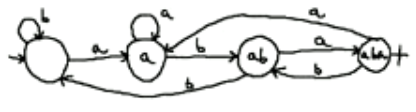
\includegraphics{t2-3.png}

\end{easylist}

\subsection{Autómatas finitos indeterministas (NFA)}
\begin{easylist}[itemize]
& Los autómatas finitos no deterministas son una extensión de los autómatas finitos deterministas. Es extraño; las ejecuciones no están unívocamente definidas. Tienen diversos caminos de ejecución que puede escoger de manera no determinista.

& Ejemplo. Tiene algo especial, el estado inicial tiene dos transiciones con $a$: una que va al propio estado y otra que va a otro estado.

\ \begin{tikzpicture}[->,>=stealth',shorten >=1pt,auto,node distance=2.8cm,semithick]

  \node[initial,state]      (A)                 {$A$};
  \node[initial,state]      (B) [right of=A]    {$B$};
  \node[initial,state]      (C) [right of=B]    {$C$};
  \node[accepting, state]   (D) [right of=C]    {$D$};

  \path (A) edge [loop above] node {$a, b$} (A)
        (A) edge              node {$a$}    (B)
        (B) edge              node {$a, b$} (C)
        (C) edge              node {$a, b$} (D);
\end{tikzpicture}

& En el último estado, no hay transiciones. Al leer un símbolo no vamos a ningún estado.
& Ejemplo de lectura de la entrada con la palabra $abbaba$. Existen diversas ejecuciones.
&& Una posible ejecución es quedarse siempre en el estado inicial. La palabra se rechazaría.
&& Otra ejecución es seguir los estados $A$, $B$, $C$ y $D$. Como no tenemos transiciones a partir del último estado, acabamos la ejecución y es una ejecución rechazadora.
&& Otra posible es hacer $abb$ en el primer estado, $a$ en el $B$, $b$ en $C$ y $a$ en $D$. En este caso sí que se aceptaría la palabra.
& Por definición, el conjunto de palabras aceptadas por el autómata es el conjunto de palabras tales que existe una ejecución aceptadora.
& En este caso, se aceptan las palabras que tienen una $a$ en la tercera posición comenzando por el final. Es decir, $[a,b]^*a[a,b]^2 = \{w \in \{a,b\}^* \colon \exists x, y \colon (w = xay \land |y| = 2)\}$.
& Es un error pensar que los autómatas finitos no deterministas tienen ``probabilidad'' de aceptar o no. Recordemos que una palabra se acepta si \textit{existe} una ejecución que llega a un estado aceptador.
& Todo autómata indeterminista se puede convertir en uno determinista que reconoce el mismo lenguaje. El autómata determinista simula todas las ejecuciones posibles del estado determinista.

& Para ello, vamos mirando cada estado adónde puede ir y lo que recuerda.
& Ejemplo (\textit{mirad el vídeo correspondiente}):
&& Indeterminista (enunciado).

\ \begin{tikzpicture}[->,>=stealth',shorten >=1pt,auto,node distance=2.8cm,semithick]

  \node[initial,state]      (A)                 {$A$};
  \node[initial,state]      (B) [right of=A]    {$B$};
  \node[initial,state]      (C) [right of=B]    {$C$};
  \node[accepting, state]   (D) [right of=C]    {$D$};

  \path (A) edge [loop above] node {$a, b$} (A)
        (A) edge              node {$a$}    (B)
        (B) edge              node {$a, b$} (C)
        (C) edge              node {$a, b$} (D);
\end{tikzpicture}

&& Determinista (resultado).

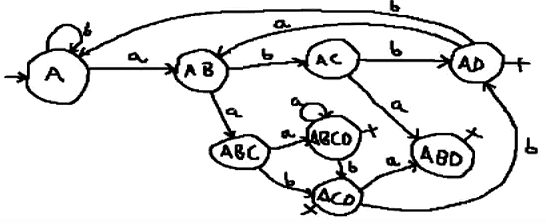
\includegraphics{t2-5.png}

\end{easylist}


\subsection{Notaciones de DFA y NFA (1)}
\subsubsection{Notaciones de DFA}
\begin{easylist}[itemize]
& Podemos usar notación por grafos.

\ \begin{tikzpicture}[->,>=stealth',shorten >=1pt,auto,node distance=2.8cm,semithick]

  \node[initial, accepting, state] (A)  {$0$};
  \node[state] (B) [right of=A] {$1$};

  \path (A) edge [loop above] node {$b$} (A)
        (B) edge [loop right] node {$b$} (B)
        (A) edge [bend left] node {$a$} (B)
        (B) edge [bend left] node {$a$} (A);
\end{tikzpicture}

& También podemos utilizar una tabla. Al principio de las filas ponemos los estados, y en el principio de las columnas ponemos los símbolos del alfabeto de entrada. Para cada casilla, indicamos el estado al que vamos a parar si, en la correspondiente fila leemos el símbolo de la correspondiente columna. Por ejemplo, si leemos una $a$ en el estado $0$, saltaremos al estado $1$. Normalmente, utilizamos $\to$ y $\dag$ para estados inicial y aceptadores, respectivamente. A veces, no se dibuja la flecha dando así a entender que el inicial es el de la primera fila.

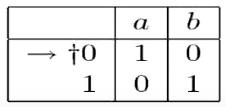
\includegraphics{t2-7.png}

& También se pueden representar por la tupla $\langle Q, \Sigma, \delta, q_0, F\rangle $.

& Podemos extender la función $\delta$ para que funcione también con palabras, no solo con símbolos del alfabeto. A esto se le llama la \textit{función de transición extendida}, y tiene la forma $\delta \colon Q \times \Sigma ^*  \to Q$.

& Intuitivamente, dado un estado y una palabra, la función de transición extendida devuelve el estado resultante de leer esta palabra a partir del estado dado.

& Por simplicidad, podemos escribir $\delta(q, a)$ por $q\cdot a$ o, simplemente, $qa$.

& Si aplicamos la palabra vacía a un estado, nos quedamos en el mismo estado: $q\lambda = q$. Es decir, $\delta(q, \lambda) = q$.

& Cualquier estado operado con una concatenación de palabras da como resultado operar primero el estado con la primera palabra y el estado resultante operarlo con la segunda palabra: $q(xy) = (qx)y$. 

& Otra propiedad: $q(a_1a_2\cdots a_n) = (\cdots ((qa_1)a_2)\cdots)a_n$.

& El lenguaje reconocido por un DFA se puede escribir como $\mathcal L (A) = \{w \colon q_0 w \in F\}$. Es decir, son todas aquellas palabras $w$ tales que, a partir del estado inicial $q_0$, llegan a un estado aceptador cualquiera (un elemento de $F$).

& También podemos definir el lenguaje reconocido por un DFA pero a partir de un estado concreto $q$ así: $\mathcal L(A, q) = \{w \colon qw \in F\}$.

& A un lenguaje se le dice \textit{regular} si y solo si existe un DFA tal que lo reconoce: $\mathcal L \in \textrm{Reg} \iff \exists A \in \textrm{DFA} \colon \mathcal L(A) = L$.
\end{easylist}

\subsubsection{Notaciones de NFA}
\begin{easylist}[itemize]
& Mismas definiciones que DFA, pero con algunos cambios. Se siguen pudiendo representar como grafos.

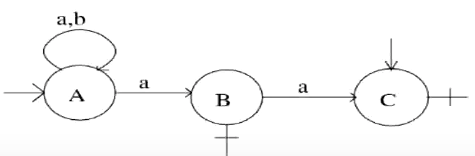
\includegraphics{t2-8.png}

& Permiten transiciones múltiplemente definidas (el estado $A$ tiene dos transiciones con la $a$), o no definidas, como pasa con la $b$ en $B$ y $C$.

& Además, admiten múltiples estados iniciales.

& Una palabra es aceptada si existe una ejecución aceptadora. Es decir, si existen un estado inicial y otro final tal que la lectura de la palabra en el estado inicial lleva al estado final.

& La representación en tabla es la misma. Puede haber más de un estado destino en cada casilla, o puede no haber ninguno.

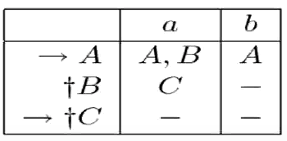
\includegraphics{t2-9.png}

\end{easylist}

\subsection{Notaciones de DFA y NFA (2)}
\subsubsection{Notaciones de NFA (continuación)}

\begin{easylist}[itemize]
& Diferencia como representación de tupla respecto los DFA: ahora no tenemos un estado inicial $q_0$, sino que podemos tener varios. Así, un NFA es una tupla $\langle Q, \Sigma, \delta, I, F\rangle$ (notad el uso de $I$ en vez de $q_0$ a diferencia de los DFA).

& Como ahora podemos ir a parar a distintos estados a partir de un estado, la función de transición también cambia su definición. Dado un estado y un símbolo, nos da como resultado un subconjunto del conjunto de estados. Es decir, $\delta \colon Q \times \Sigma \to 2^Q$.

& También notamos que $\delta \subseteq Q \times \Sigma \times Q$.

& Podemos extender la función de transición para aplicarla a un conjunto de estados y un símbolo: $\delta \colon 2^Q \times \Sigma \to 2^Q$.

& La imagen de un par (conjunto de estados, símbolo) es la unión de las imágenes de cada estado del conjunto y el símbolo. Es decir, $\delta(\{q_1, \dots, q_m\}, a) = \delta(q_1, a) \cup \dots \cup \delta(q_m, a)$. Intuitivamente, esto nos dice a qué estados podemos ir a parar si nos encontramos en algún estado de un conjunto fijado.

& Podemos extender la función de transición todavía más a conjuntos de estados y palabras cualesquiera, y no necesariamente a símbolos del alfabeto. Esto es, $\delta \colon 2^Q \times \Sigma^* \to 2^Q$. Esto se hace de manera totalmente análoga al caso de los DFA.

& La palabra vacía, $\lambda$, nos deja donde está: $\delta(\{q_1, \dots, q_m\}, \lambda) = \{q_1, \dots, q_m\}$.

& Y, al aplicar sobre la concatenación, primero se aplica sobre la primera palabra y, después, sobre la segunda: $\delta(\{q_1, \dots, q_m\}, xy) = \delta(\delta(\{q_1, \dots, q_m\}, x), y)$.

& Lenguaje aceptado por un FA: $\mathcal L(A) = \{w \colon \delta(I, w) \cap F \neq \varnothing\}$. Esto es, el conjunto de palabras para las que existe una ejecución aceptadora comenzando a partir de alguno de los estados iniciales.

& El proceso de determinización es sencillo a partir de la tabla.

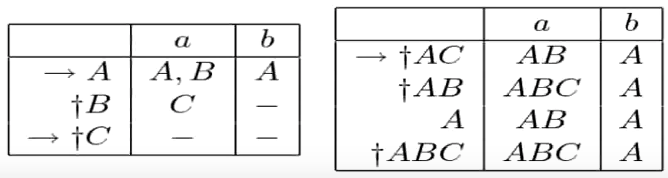
\includegraphics[width=10cm]{t2-10.png}

& Ponemos, como estados aceptadores, aquellos que incluyen en su nombre algún estado aceptador de la tabla de la izquierda.
\end{easylist}

\subsubsection{\texorpdfstring{$\lambda$}{Lambda}-NFA}
\begin{easylist}[itemize]
& Una $\lambda$-transición es una transición etiquetada con la palabra vacía.

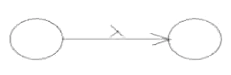
\includegraphics{t2-11.png}

& Esta transición se puede efectuar o no, de manera que los $\lambda$-NFA pueden tener varias ejecuciones diferentes para una misma palabra, como ya pasaba en los NFA en general.

& La noción de aceptación de una palabra por parte de un $\lambda$-NFA es la misma que para NFA. Es decir, decimos que el autómata acepta una palabra si existe una ejecución aceptadora para esta palabra.

& Los $\lambda$-NFA son igual de expresivos que los DFA. Es decir, tan solo pueden reconocer lenguajes regulares.

& Cualquier autómata con $\lambda$-transiciones se puede convertir en uno sin $\lambda$-transiciones que reconozca el mismo lenguaje.

& Para poder efectuar esta conversión, tenemos que añadir algunas cosas al autómata. 

& $\delta \subseteq Q \times (\Sigma \cup \{\lambda\}) \times Q$.

& Si hay algún camino con símbolos $\lambda$, podemos anticiparnos y añadir a mano otra transición, de manera que cuando borremos los $\lambda$ todavía tengamos el camino. Notamos que igual podíamos llegar de un estado a otro ejecutando las $\lambda$-transiciones.

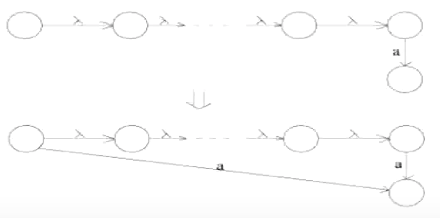
\includegraphics{t2-12.png}

& Si tenemos un camino de $\lambda$-transiciones que lleva hacia un estado aceptador, entonces ponemos el primero como aceptador, anticipándonos, de nuevo.

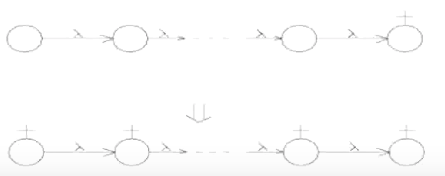
\includegraphics{t2-13.png}

& Hecho esto, ya podemos borrar las $\lambda$-transiciones del $\lambda$-NFA y obtenemos un NFA equivalente.
\end{easylist}


\subsection{Operaciones sobre Reg (1)}

Cuando operamos dos lenguajes regulares con ciertas operaciones conocidas, el resultado es otro lenguaje regular. En esta sección veremos la intersección, unión y complementario de lenguajes.

\subsubsection{Intersección y unión}
\begin{easylist}[itemize]
& Los lenguajes regulares son cerrados por intersección y unión. Esto es, que si $L_1, L_2 \in \textrm{Reg}$, entonces $L_1 \cap L2$ y $L_1 \cup L_2$ pertenecen a $\textrm{Reg}$.

& Vamos a analizar un ejemplo.

El autómata de arriba reconoce las palabras sobre $\{a,b\}$ con un número par de $a$s, y el de abajo reconoce las palabras sobre $\{a,b\}$ con un número par de $b$s.

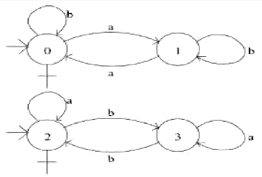
\includegraphics{t2-14.png}

& Para obtener el autómata \textit{intersección}, construiremos un autómata que simule estos dos.


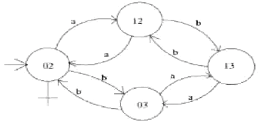
\includegraphics{t2-15.png}

& Este autómata recuerda en qué estado se encuentran los dos anteriores con una palabra leída hasta el momento.

& Por ejemplo, cuando no hemos leído nada en ningún autómata, debemos recordar que ambos autómatas se encuentran en sus estados iniciales. Por eso, recordamos los estados 0 y 2 respectivamente.

& Si leemos una $a$, en el primer autómata nos vamos al estado $1$, y en el segundo, al $2$. Por tanto, iremos al estado $12$.

& Si leemos una $a$ desde $12$, como desde $1$ pasamos a $0$, y desde $2$ seguimos quedándonos en $2$, pasamos, pues, al estado $02$. Y así sucesivamente.

& Si queremos reconocer la intersección, debemos aceptar palabras tales que, en ambos autómatas, nos lleven a estado aceptador. Por eso, ponemos como estado aceptadores aquellos que recuerden que ambos autómatas se encuentran en estado aceptador. En el caso anterior, solo $02$ es aceptador.

& Si quisiésemos reconocer la unión, la elección de los estados aceptadores es diferente. Aceptamos las palabras que aceptan alguno de los dos autómatas. Los estados aceptadores serán los que recuerden que alguno de los dos autómatas ha llegado hasta un estado aceptador. En nuestro caso, $02$, $12$ y $03$ serían aceptadores.

& Vamos a ver lo anterior, ahora, de manera formal. Supongamos que tenemos los autómatas $A_1 = \langle Q_1, \Sigma, \delta_1, q_{01}, F_1\rangle$ y $A_2 = \langle Q_2, \Sigma, \delta_2, q_{02}, F_2\rangle$.

& Definimos el autómata intersección, denotado abusivamente por $A_1 \cap A_2$, como $\langle Q_1 \times Q_2, \Sigma, \delta, \langle q_{01}, q_{02}\rangle, F_1 \times F_2\rangle$. Este autómata tiene como estados las parejas de estados de los dos autómatas anteriores, como estado inicial la pareja de estados iniciales de los dos autómatas anteriores, y como estados aceptadores, todas las parejas de estados aceptadores de los dos autómatas anteriores, y, como función de transición, $\delta(\langle q_1, q_2\rangle, a) = \langle\delta_1(q_1, a), \delta_2(q_2, a)\rangle$. Esto es, a cada par de estados de $A_1$ y $A_2$ les asigna sus estados transición correspondientes por $\delta_1$ y $\delta_2$.

& Esta descripción formal no se corresponde exactamente a la idea anterior del dibujo, porque algunas parejas de estados sean inaccesibles. En estos casos, no las consideraremos.

& Lo más recomendable para hacer la intersección de autómatas es mediante tablas.

& \textit{$\triangle$ Ejercicio: transformar a tablas los dos autómatas anteriores}.

& Definimos el autómata intersección, denotado abusivamente por $A_1 \cup A_2$ de manera parecida al autómata unión. En este caso es $\langle Q_1 \times Q_2, \Sigma, \delta, \langle q_{01}, q_{02}\rangle, (F_1 \times Q_2) \cup (Q_1 \times F_2)\rangle$. La única diferencia, como hemos visto antes, será en cuáles son los estados acepadores. En este caso, necesitamos, como estados aceptadores a una pareja tal que, o bien el primero es aceptador del primer autómata o bien el segundo es aceptador del segundo autómata.

& Estos autómatas reconocen los lenguajes intersección y unión. Esto es, $\mathcal L(A_1 \cap A_2) = \mathcal (A_1) \cap \mathcal L (A_2)$ y $\mathcal L(A_1 \cup A_2) = \mathcal (A_1) \cup \mathcal L (A_2)$.

& Los lenguajes regulares también son cerrados por la operación de complementario. Esto es, $L \in \textrm{Reg} \implies \bar L \in \mathrm{Reg}$.
\end{easylist}


\subsubsection{Complementario}
\begin{easylist}[itemize]
& Dado un autómata $A = \langle Q, \Sigma, \delta, q_0, F\rangle$, su complementario es $\bar A = \langle Q, \Sigma, \delta, q_0, Q - F\rangle$. Este autómata acepta las palabras que no acepta $A$, y viceversa. Lo único que hacemos es intercambiar estados aceptadores y rechazadores en la descripción formal del autómata.

& $\overline{\mathcal L(A)} = \mathcal L(\bar A)$.

& Esta idea no funciona con autómatas indeterministas. Esto se debe a que en autómatas indeterministas, una palabra es aceptadora si existe alguna ejecución que lleva a un estado aceptador. Pero puede pasar que una palabra llegue a estados aceptadores y rechazadores. Por esta razón, antes de aplicar la operación de complementario hay que determinizar el autómata.
\end{easylist}

\subsection{Operaciones sobre Reg (2)}
\subsubsection{Concatenación}
\begin{easylist}[itemize]
& Los lenguajes regulares son cerrados por la operación de concatenación. Es decir, $L_1, L_2 \in \text{Reg} \implies (L_1 \cdot L_2) \in \text{Reg}$. Esto es, que si existen autómatas para ambos lenguajes, entonces también existe el autómata del lenguaje de su concatenación.

& Para convencernos de ello, supongamos que el autómata de la izquierda reconoce $L_1$, y, el de la derecha, $L_2$. 

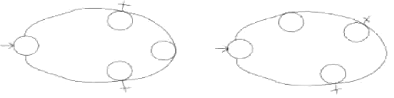
\includegraphics{t2-16.png}


& Recordemos que el lenguaje concatenación es el formado por aquellas palabras que son concatenación de palabras formadas por concatenación de una palabra de $L_1$ con una palabra de $L_2$.

& Para construir un autómata de su concatenación, hay que añadir $\lambda$-transiciones desde los estados aceptadores del primer autómata hasta el estado inicial del segundo autómata. Además, los estados aceptadores del primer autómata dejan de ser aceptadores en el nuevo autómata. Y el estado inicial del segundo autómata deja de serlo.

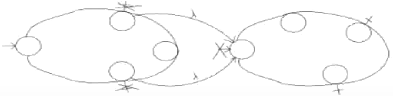
\includegraphics{t2-17.png}


& Justificación de que el autómata anterior reconoce el lenguaje concatenación. Por un lado, cualquier palabra $w$ del lenguaje concatenación se puede partir en dos partes, $w_1$ y $w_2$ de $L_1$ y $L_2$, respectivamente. Como $w_1$ es de $L_1$, esta nos lleva del estado inicial del autómata de $L_1$ a un aceptador del primer autómata. Esta ejecución se puede reproducir en el autómata concatenación, y ejecutar después la $\lambda$-transición correspondiente hacia el estado inicial del segundo autómata. Análogamente, $w_2$ nos lleva a un estado aceptador del segundo autómata. Esta ejecución se puede realizar de la misma manera en el autómata concatenación, resultando así que la composición con la anterior ejecución nos da una ejecución aceptadora de $w$. Así pues, toda palabra del lenguaje concatenación es aceptada por este nuevo autómata.

& Nos falta justificar el sentido contrario, esto es, que toda palabra aceptada por el autómata es del lenguaje concatenación. Pero esto es sencillo, pues toda ejecución aceptadora en el autómata concatenación ha de pasar en algún momento por alguna $\lambda$-transición. Por tanto, esta palabra tendrá una ejecución desde el estado inicial del primer autómata hasta un estado aceptador del primer autómata, y lo que queda de la palabra nos lleva desde el estado aceptador del segundo autómata a un estado final del segundo autómata. Esto justifica que la palabra se puede partir en una subpalabra de $L_1$ y de $L_2$. Por tanto, la palabra es del lenguaje concatenación.

\end{easylist}


\subsubsection{Estrella}
\begin{easylist}[itemize]
& Vamos a ver ahora que los lenguajes regulares son cerrados por la operación estrella. Esto es, que si existe un autómata que reconoce un lenguaje, entonces también existe otro que reconoce su estrella: $L \in \textrm{Reg} \implies L^* \in \textrm{Reg}$.

& Recordamos que la estrella de un lenguaje $L$ es el lenguaje de las palabras que se obtienen al concatenar palabras de $L$. Por tanto, queremos aceptar subpalabras que nos lleven del estado inicial a algún estado aceptador. 

& Para reconocer el lenguaje estrella, solo tenemos que añadir $\lambda$-transiciones entre todos los estados aceptadores al estado inicial.

& Además, si el estado inicial del autómata no es aceptador, hay que añadir un estado inicial adicional que sea aceptador, para aceptar también la palabra vacía.

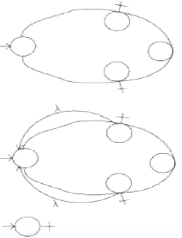
\includegraphics{t2-18.png}


& \textit{$\triangle$ Ejercicio: justificar que el autómata estrella reconoce la estrella del lenguaje original}.
\end{easylist}

\subsubsection{Reverso}
\begin{easylist}[itemize]
& Vamos a ver ahora que los lenguajes regulares son cerrados por la operación reverso. Esto es, que si existe un autómata que reconoce un lenguaje, entonces también existe otro que reconoce su reverso: $L \in \textrm{Reg} \implies L^R \in \textrm{Reg}$.

& Sea el primer autómata uno que reconozca $L$. Las palabras de $L$ son las que nos llevan del estado inicial a algún estado aceptador. Por tanto, una palabra de $L^R$ nos llevaría de un estado aceptador al estado inicial siguiendo las flechas en sentido inverso. 

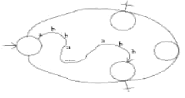
\includegraphics{t2-19.png}


& Basándonos esta idea, definimos el estado reverso de esta manera. Si $A = \langle Q, \Sigma, \delta, q_0, F\rangle$, entonces $A^R = \langle Q, \Sigma, \{qa \to q'|(q'a\to q) \in \delta\}, F, \{q_0\}\rangle$. El autómata reverso tiene los mismos estados y el mismo alfabeto que el original; sus transiciones son las del original pero giradas. Es decir, si en el original íbamos de $q'$ a $q$ después de leer una palabra $a$, en el reverso vamos de $q$ a $q'$ después de leer la palabra $a$. Además, se intercambian estados iniciales y aceptadores. El conjunto de estados aceptadores contiene ahora, únicamente, el estado inicial del autómata original.

& \textit{$\triangle$ Ejercicio: justificar que $\mathcal L(A^R) = (\mathcal L(A))^R$.}
\end{easylist}


\subsubsection{Técnica de obtención de DFA o NFA por descomposición}
\begin{easylist}[itemize]
& Vamos a ver una técnica que permite construir un autómata que reconoce lenguajes complejos. Para eso nos basaremos en las operaciones de clausura que hemos visto anteriormente.

& La idea consiste en formalizar el lenguaje, y después ir descomponiendo esta formalización mediante operaciones intermedias hasta que el lenguaje de partida sea descrito en función de lenguajes sencillos para los cuales sea fácil obtener un autómata autómaticamente. No es una técnica infalible.

& Ejemplo. Queremos obtener el autómata que reconozca el lenguaje de las palabras sobre $a$ y $b$ tales que, a la derecha de toda $a$ queda una palabra con un número par de $b$s. Esto es, el lenguaje $L = \{w \in \{a,b\}^* \colon \forall x,y \colon (w = xay \implies |y|_b \in \dot 2\}$.

& Encontrar un autómata directamente es difícil. La formalización anterior incluye un cuantificador universal. Habitualmente, es más sencillo encontrar autómatas para propiedades existencialmente cuantificadas. Por este motivo, calcularemos el lenguaje complementario a $L$, formalizable por $\bar L = \{w \in \{a,b\}^* \colon \exists x, y \colon (w = xay \land |y|_b \notin \dot 2\}$.\footnote{Se ha aplicado que $\neg \forall x (p(x)) \equiv \exists x (\neg p(x))$ y la definición de implicación: $p \to q \equiv \neg p \lor q$.} Como los lenguajes son cerrados por complementario, si encontramos un autómata para $\bar L$, podremos convertirlo en uno para $L$. 

& Nótese que el existencial liga bien con la noción de aceptación en autómatas no deterministas, pues nos preguntamos por la existencia de una ejecución hacia un estado aceptador. Sería suficiente pues, con un autómata indeterminista que, de manera no determinista escoja una $a$, y después compruebe que lo que queda es un número impar de $b$.

& De todas maneras, todavía se puede descomponer más el autómata. $\bar L = \{a,b\}^* \{a\} \{y \in \{a,b\}^* \colon |y|_b \notin \dot 2\}$. En definitiva, tenemos que $w$ se parte en tres subpalabras. La primera subpalabra es una cualesquiera, la segunda es una $a$ y la tercera tiene un número impar de $b$s. Así pues, $\bar L$ es la concatenación de estos tres lenguajes. Ahora sí que podemos obtener autómatas sencillos.

& \textit{$\triangle$ Ejercicio: dibujar el autómata para $L$ a partir de la descomposición anterior}.


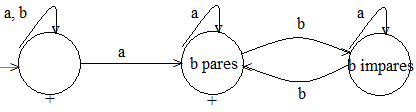
\includegraphics{t2-20.png}

& Observación: también podríamos haber calculado el reverso fácilmente, como $L^R = \{w \in \{a,b\}^* \colon \forall x, y \colon (w = xay \implies |x|_b \in \dot 2\}$. Esto es, las palabras que tienen un número impar de $b$s seguidas de $a$ y de una palabra cualquiera.

\end{easylist}


\subsection{Operaciones sobre Reg (3)}


\subsubsection{Morfismo directo}
\begin{easylist}[itemize]
& Si hay un autómata que reconoce un lenguaje, entonces también hay otro que reconoce la imagen de este lenguaje por un morfismo: $L \in \textrm{Reg} \land \sigma(xy) = \sigma(x)\sigma(y) \implies \sigma(L) \in \textrm{Reg}$.

& La construcción la haremos mediante un ejemplo. Suponemos que tenemos el morfismo $\sigma \colon \{a,b,c\}^* \to \{0, 1\}^*$ tal que $\sigma(a) = 01$, $\sigma(b) = 1$ y $\sigma(c) = \lambda$ y el autómata de arriba de la figura para $L$. El autómata que reconoce $\sigma(L)$ es el de abajo.

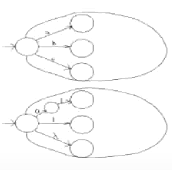
\includegraphics{t2-21.png}

& En el nuevo autómata:
&& Si tenemos una transición de tamaño uno, simplemente renombramos las etiquetas.
&& Si tenemos una transición con imagen de mayor tamaño, entonces añadimos suficientes estados intermedios nuevos.
&& Por último, si la imagen de la transición tiene tamaño cero (situación en la que la imagen es $\lambda$), entonces transformamos la transición en una $\lambda$-transición.

& Aplicamos estos cambios a todas las transiciones del autómata original.

& \textit{$\triangle$ Ejercicio: justificar que este nuevo autómata realmente reconoce el morfismo del lenguaje original.}
\end{easylist}

\subsubsection{Morfismo inverso}
\begin{easylist}[itemize]
& Los lenguajes regulares también son cerrados por morfismo inverso. Es decir, si existe un autómata que reconoce un lenguaje, entonces también hay otro que reconoce el conjunto imagen de este por un morfismo. Es decir, $L \in \mathrm{Reg} \land \sigma \colon \Sigma_1^* \to \Sigma_2^* \land \sigma(xy) = \sigma(x)\sigma(y) \implies \sigma^{-1} (L) \in \mathrm{Reg}$.

& Recordemos que la antiimagen de un conjunto $L$ es el conjunto de elementos cuya imagen está en $L$.

& A partir de un autómata $A = \langle Q, \Sigma_2, \delta, q_0, F\rangle$ que reconoce $L$, veamos cómo construir un autómata que reconozca $\sigma^{-1}(L)$.

& El autómata antiimagen tiene los mismos estados que $A$, pero su alfabeto es el correspondiente al dominio de $\Sigma_1$. Tendrá los mismos estados aceptadores y estado inicial que $A$, y la principal diferencia está en las reglas. $\sigma^{-1}(A) = \langle Q, \Sigma_1, \delta', q_0, F\rangle$.\footnote{En el minuto 2:15 del vídeo hay un error en esta definición. Aquí está correctamente escrita.}

& Hay que definir $\delta'$ para parejas (estado de $Q$, símbolo de $\Sigma_1$), obteniendo como resultado otro estado de $Q$: $\delta' \colon Q \times \Sigma_1 \to Q$.

& El estado al que iremos a parar desde $q$ después de leer $a$ lo definimos como el estado al que íbamos a parar en el autómata original después de leer la imagen original desde $q$. Esto es, $\delta'(q,a) = \delta(q, \sigma(a))$. Nótese que la imagen de $a$, $\sigma(a)$ no necesariamente tiene tamaño 1. No obstante, esto no es un problema, porque podíamos extender la definición de $\delta$ para pares (estado, palabra).

& Formalmente, $\sigma^{-1}(L) = \sigma^{-1}(\mathcal L(A)) = \mathcal L (\sigma^{-1}(A))$.\footnote{Consultad \url{http://youtu.be/L8HtVewJfzM} a partir del minuto 3:23 para la demostración (totalmente formal y nada intuitiva) de esta propiedad.}
\end{easylist}


\subsection{Minimización de DFA (1)}
\begin{easylist}[itemize]
& En esta sección y en las siguientes veremos que, en todos los DFA que reconocen un lenguaje fijado, hay uno concreto que tienen menos estados estados que cualquiera de los otros, y que llamaremos \textit{DFA mínimo}.

& Empezamos analizando este ejemplo de DFA.

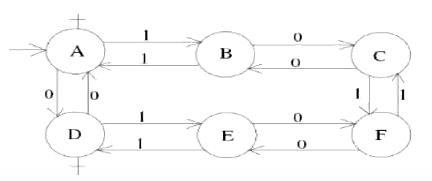
\includegraphics{t2-22.png}

& Imaginemos que estamos en medio de una ejecución y que nos encontramos, o bien en el estado $A$, o bien en el $D$, pero no sabemos en cuál de los dos. Si de repente la ejecución acaba, en ambos casos aceptaremos. En caso contrario, si leemos un $0$, seguimos en $A$ o $D$, sin saber en cuál. Si leemos un $1$, pasaremos al estado $B$ o $E$; no sabemos cuál. Si la ejecución acaba, sea cual sea el caso, acabamos. En cambio, si leemos un $0$, iremos a $C$ o $F$, sin saber en cuál. Si acaba la ejecución, rechazamos. En caso contrario, si ahora leemos un $1$, iremos a $C$ o $F$ sin saber a cuál, etc.

& Todo este discurso nos puede servir para intuir que los estados $A$ y $D$ son equivalentes en el sentido de que las palabras aceptadas empezando desde $A$ son las mismas que aquellas aceptadas empezando desde $D$. Los estados $B$ y $E$, y $C$ y $F$ son también equivalentes en este sentido.

& Esta noción de equivalencia nos servirá para reducir el tamaño del DFA. Por ejemplo, intuitivamente, parece que la transición de $E$ a $D$ con un $1$ la podríamos desviar hacia $A$, ya que desde $A$ se reconoce el mismo lenguaje desde $D$. Y la transición de $A$ a $D$ la podríamos redirigir también hacia $A$ (un bucle). Así $D$ ya no sería accesible y lo podríamos borrar.

& Vamos a concretar estas ideas con el objetivo de reducir el tamaño de un DFA hasta encontrar el DFA mínimo reconociendo el mismo lenguaje.

& Definimos la siguiente relación entre estados de $A = \langle Q, \Sigma, \delta, q_0, F \rangle$ que denotamos por $q\sim_A q'$ o como $q \sim q'$ así: dos estados $q$ y $q'$ son equivalentes o indistinguibles ($q \sim q'$) si los lenguajes reconocidos desde ellos son equivalentes: $\mathcal L (A, q) = \mathcal L (A, q')$. Esto es, que para toda palabra $w$, desde $q$ llegamos a estado aceptador después de leer $w$ si y solo si desde $q'$ llegamos a estado aceptador después de leer $w$: $\forall w \in \Sigma^* \colon (qw \in F \iff q'w \in F )$.

& No es difícil comprobar que la relación anterior es de equivalencia: es reflexiva, simétrica y transitiva.

& Recordamos que, siempre que tenemos una relación de equivalencia sobre un conjunto, se puede hablar del conjunto cociente, $Q / \sim$, que es la partición en clases de equivalencia. En nuestro ejemplo anterior,  el conjunto cociente es $Q/ \sim = \{\{A, D\},\{B, E\}, \{C, F\}\}$.

& La clase de equivalencia de un elemento $q$ es $[q]$. Así, $[A] = [D] = \{A, D\}$ en el ejemplo anterior.

& Vamos a demostrar que, cuando dos estados son indistinguibles o equivalentes, después de leer el mísmo símbolos desde ellos, vamos a parar a una pareja de estados que también son equivalentes. Esto es que si $q \sim q'$ (también se puede escribir como $[q] = [q']$, entonces, $\forall a \in \Sigma$, $qa \sim q'a$; o lo que es lo mismo, que $[qa] = [q'a]$.\footnote{Hay un error en el minuto 3:34 del vídeo \url{https://youtu.be/QN7V3fVZRNI} sin notificar. Las clases de equivalencia resultantes de $q$ y $q'$ son iguales, pero no están relacionadas por $\sim$.}

& Demostramos esta propiedad:
&& Comenzamos con la hipótesis de que $q$ y $q'$ son equivalentes ($q \sim q'$) y sea $a$ un símbolo cualquiera de $\Sigma$.
&& Por definición de equivalencia, tenemos que $\forall w \colon (qw \in F \iff q'w \in F)$.
&& En particular, cualquier palabra que empiece por $a$ también lo verificará: $\forall w \colon (q(aw) \in F \iff q'(aw) \in F)$.
&& Esto implica que cualquier palabra nos lleva a estao aceptador desde el estado $qa$ si y solo si nos lleva a estado aceptador desde el estado $q'a$: $\forall w\colon ((qa)w \in F \iff (q'a)w \in F)$.
&& Pero esto es precisamente $qa \sim q'a$, como queríamos demostrar.

& Dicho de otra manera, $\forall w \in \Sigma^* \colon ([q] = [q'] \implies [qw] = [q'w])$.

& El autómata cociente se deduce de las propiedades anteriores: $A/\sim = \langle Q/\sim, \Sigma, \{[q]a \to [qa]\colon q \in Q, a \in \Sigma\}, [q_0], \{[q] \colon q \in F\}\rangle$. Esto es, los estados son las clases de equivalencia, el alfabeto es el mismo, el estado inicial es la clase del estado inicial y los estados aceptadores son las clases de aquellos estados que eran aceptadores. La función de transición se define como aparece en esta definición.

& Este autómata reconoce el mismo lenguaje que el autómata original: $\mathcal L(A) = \mathcal L (A/\sim)$. Vamos a demostrarlo:

&& Esto es equivalente a decir que para toda palabra $w = a1\dots a_n$ de $\Sigma^*$, $q_0w \in F$ si y solo si $[q_0]w \in \{[q] \colon q \in F\}$, o, dicho de otra manera, que la palabra es aceptada en $A$ si y solo si es aceptada en $A / \sim$.

&& Aplicando la definición de función de transición en $A / \sim$, podemos deducir que el estado al que se va a parar después de leer $w$ desde la clase del estado inicial del autómata cociente; esto es, $[q_0]$, es la clase del estado $q_0 w$, $[q_0w]$. En definitiva: $[q_0]w = [q_0 w]$. La demostración va como sigue:

$[q_0]w = [q_0](a_1 \dots a_n) = ([q_0]a_1)(a_2 \dots a_n) = [q_0 a_1](a_2 \dots a_n) =$

$= ([q_0 a_1]a_2) (a_3 \dots a_n) = [q_0 a_1 a_2](a_3 \dots a_n) = \dots = [q_0 w]$.

&& Por tanto, hay que demostrar que $q_0 w \in F \iff [q_0w] \in \{[q] \colon q\in F\}$; pero esto es obvio, ya que, por la definición del autómata cociente, la clase de un estado es aceptadora si este estado es aceptador. Esto acaba con la demostración.

& Volviendo con el ejemplo anterior, este es el autómata cociente equivalente.

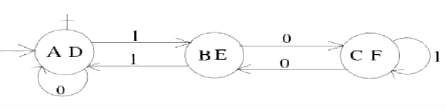
\includegraphics{t2-23.png}

\end{easylist}




\subsection{Minimización de DFA (2)}
\begin{easylist}[itemize]
& En esta sección veremos cómo calcular la partición en clases de estados indistinguibles de un DFA.

& Sea $A = \langle Q, \Sigma, \delta, q_0, F\rangle$. Recordamos que dos estados son indistinguibles cuando los respectivos lenguajes reconocidos desde $q$ y $q'$ coinciden, o, alternativamente, que cualquier palabra nos lleva a estado aceptador desde $q$ si y solo si lo hace desde $q'$. Más formalmente: $q \sim_A q' \equiv q \sim q' \equiv \mathcal L(A,q) = \mathcal L(A, q') \equiv \forall w \in \Sigma^* \colon (qw \in F \iff q'w \in F)$.


& Para ver qué parejas de estados son equivalentes, comprobamos esta propiedad. Empezaremos con palabras de longitud 0, después, de longitud 1, y así sucesivamente.

& Con esta finalidad nos será útil construir una relación de equivalencia para cada longitud.

& Con $q\sim_{A, k} q'$ (o simplemente $q \sim_k q'$ si se sobreentiende el autómata $A$) notamos que $q$ y $q'$ son dos estados $k$-indistinguibles. Por definición, dos estados son $k$-indistinguibles si $\mathcal L(A, q) \cap \{w \in |w| \leq k\} = \mathcal L(A, q') \cap \{w \in |w| \leq k\}$. Esto es, si los lenguajes reconocidos por ambos coinciden considerando solo las palabras de longitud hasta longitud $k$. Equivalentemente, también $q \sim q'$ si $\forall w \in \Sigma^*$ tenemos que $|w| \leq k \implies (qw \in F \iff q'w \in F)$.

& La $k$-indistinguibilidad es una relación de equivalencia.

& Tampoco es difícil convencerse que dos estados son indistinguibles si son $k$-indistinguibles para todo natural $k$: $q \sim q' \iff \forall k \geq 0 \colon q \sim_k q'$.

& La $k$-indistinguibilidad se puede definir también recursivamente. Si $k = 0$ (la palabra a leer será $\lambda$, y, por tanto, no nos movemos del estado) entonces $q\sim_0 q' \equiv (q \in F \iff q' \in F)$ es decir: o bien los dos son aceptadores o bien los dos son rechazadores.

& Para $k \geq 1$, $q \sim_k q'$ es equivalente a $q\sim_{k-1} q'$ y $\forall a \in \Sigma \colon (qa \sim_{k-1} q'a)$. Esto es, que dos estados $q$ y $q'$ son $k$-indistinguibles si son $k-1$ indistinguibles y, para todo símbolo $a$, la pareja de estados a la que vamos a parar leyendo $a$ también tiene que ser $k-1$-indistinguibles; pues si se pudieran distinguir con una palabra de longitud $k-1$, entonces $q$ y $q'$ se podrían distinguir con una palabra de longitud $k$.

& Podemos utilizar la definición recursiva anterior para calcular $Q/\sim$ o, abusivamente, $\sim$, en el autómata ya visto que tenéis a continuación.

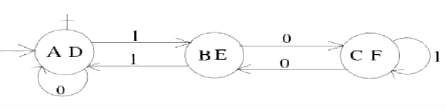
\includegraphics{t2-23.png}

& La partición en 0-indistinguibles es la partición en, por un lado los estados aceptadores y, en por el otro, los rechazadores.

$\sim_0 \colon \{A,D\} \{B, C, E, F\}$.

& Ahora, miramos dos a dos en cada conjunto para ver si vamos a parar a estados de la misma clase. Si lo hacen, no tocamos las particiones. Sino, agregamos particiones.

& La partición $\{A, D\}$ no la podemos separar, porque:
&& Si leemos un $0$, desde $A$ llegamos a $[A]$, y desde $D$ también.
&& Si leemos un $1$, desde $A$ llegamos a $[B]$, y desde $D$ también (recordad que $[B] = \{B, C, E, F\}$.

& En cambio, si comparamos $B$ y $C$, si leemos un $0$ nos quedamo en $[B]$, pero si leemos un $1$, en $B$ vamos a $[A]$ y en $C$ nos quedamos en la misma clase $[F]$. Por tanto, los separamos.

& Con $C$ y $E$ por ejemplo, si leemos un $0$ vamos a parar a $[B]$ y a $[F]$, que ya hemos visto que pertenecen a clases diferentes.

En definitiva, $\sim_1 : \{A, D\}\{B, E\}\{C, F\}$.

& Para $\sim_2$ ya no podemos refinar más las particiones (porque ya no podemos reducir más las particiones).

& Por tanto, $\sim_k \colon \{A, D\}\{B, E\}\{C, F\}$, para toda $k \geq 1$.

& Cuando $\sim_k = \sim_{k+1}$, ya no cambia más.

& No se puede refinar un DFA más del número de estados que contiene.

& En definitiva, $\sim \colon \{A, D\}\{B, E\}\{C, F\}$, también llamado \textit{conjunto cociente}.

\end{easylist}

\subsection{Minimización de DFA (3)}
En esta sección se explica por qué el método empleado en la sección anterior para generar DFA mínimos realmente genera DFA mínimos. Esto es, que dados dos autómatas minimizados $A_1$ y $A_2$ que describen el mismo lenguaje, entonces forzosamente $A_1$ y $A_2$ son iguales excepto por renombramiento de los estados por una biyección total $f$.

No resulta de utilidad transcribir toda la demostración; consultad el vídeo correspondiente, que es \url{https://youtu.be/ON1DM6EBX6Y}.
\section{Expresiones regulares}

\subsection{Expresiones regulares (1)}
\begin{easylist}[itemize]
& Una expresión regular sobre un alfabeto usa los operadores binarios suma y producto y el operador unario estrella.

& El producto se denota sin escribir nada, y la estrella se expresa de forma similar a la exponenciación.

& Las expresiones básicas son, o bien símbolos del alfabeto, o bien $\Lambda$.

& Una expresión regular se interpreta como un lenguaje del siguiente modo:
    && Cada símbolo del alfabeto se interpreta como el lenguaje que sólo contiene ese símbolo.
    && El lenguaje de la palabra vacía, $\Lambda$, se interpreta como $\{\lambda\}$.
    && La suma se interpreta como unión.
    && El producto se interpreta como concatenación.
    && La estrella se interpreta como la operación estrella de lenguajes.

& Ejemplo: $a + bc^* (a + b)^* + \Lambda$ es una expresión regular que describe el lenguaje $\{a\} \cup [\{b\} \cdot \{c\}^* \cdot (\{a\} \cup \{b\})^*] \cup \{\lambda\}$.
    
& Así, las expresiones regulares son un método de representación de lenguajes. De hecho, de forma abusiva, identificaremos la expresión con el lenguaje representado.

& Es obvio que toda expresión regular representa un lenguaje regular, ya que los lenguajes regulares son cerrados por unión, concatenación y estrella, y existen autómatas triviales que reconocen a un solo símbolo o a la palabra vacía.

& Lo que no es tan obvio es que todo lenguaje regular se puede representar mediante una expresión regular. Es decir, para todo autómata existe una expresión regular que representa el lenguaje reconocido por el autómata. Para demostrar esto, necesitamos algunos contenidos teóricos.

& Suponemos la ecuación $X = AX + B$, donde $A$ y $B$ son lenguajes concretos y $X$ es una variable con rango en los lenguajes. Queremos saber las soluciones de la ecuación. Es decir, aquellos que, al sustituir $X$ por uno de ellos, hace la igualdad cierta.

& El \textit{lema de Arden} nos explica cómo tratar con esta igualdad en tres pasos.
&& La primera solución es $X = A^*B$.

    &&& Demostración: $A(A^*B) + B = A^+B + \Lambda B = (A^+ + \Lambda)B = A^* B$.

&& Cualquier otra solución $L$ contiene a $A^*B$. Esto es, $\forall L \colon (L = AL + B \implies A^*B \subseteq L)$.
    
    &&& Demostración: por cumplir la ecuación, $L$ contiene a $B$, $B \subseteq L$; por el mismo motivo $L$ contiene a $AL$ y, por tanto, a $AB$: $AB\subseteq AL \subseteq L$.
    
    &&& Similarmente, como $L$ contiene a $AL$ y a $AB$, entonces contiene a $A(AB)$, que es $A(A^2 B)$. Así, sucesivamente, vemos que $\forall n\colon(A^n B \subseteq L)$.
    &&& Esto concluye que $A^*B \subseteq L$.

&& Finalmente, vemos que, si $A$ no contiene la palabra vacía, entonces la única solución de la ecuación es $A^* B$. Esto es, $\lambda \notin A \implies \forall L \colon (L = AL + B \implies L = A^*B)$.
    
    &&& Lo demostramos por reducción al absurdo, suponiendo que $\lambda \notin A$, y que existe una solución a la ecuación diferente de $A^* B$: $L = AL + B \land L \neq A^* B$.
    
    &&& Como toda solución de la ecuación contiene a $A^* B$, para que $L$ y $A^*B$ sean distintos, tiene que haber una palabra $w$ que no esté en $A^* B$: $w \in L - A^* B$. Escogemos una palabra de longitud mínima ($|w|$ mínima) cumpliendo esta condición.
    
    &&& Por la ecuación, esto es $w \in (AL + B) - B$; pero, entonces, $w \in AL$.
    
    &&& Así pues, $w$ se puede construir por concatenación de una palabra de $w_1$ de $A$ con una palabra de $w_2$ de L.
    
    &&& Como $w \notin A^* B$ por hipótesis, entonces $w_w \notin A^* B$, y como $\lambda \notin A$, entonces $|w_2| < |w|$.
    
    &&& Así, hemos visto que $w_2 \in L - A^* B$, pero $|w_2| < |w|$. Esto contradice la elección mínima de $w$.
    
& Volvemos al objetivo principal: convertir un autómata en una expresión regular mediante un ejemplo.

& Queremos la expresión regular del lenguaje $L = \{w \in \{0,1\}^* \colon \mathrm{valor}_2 (w) \in \dot 3\}$; esto es, de las palabras binarias múltiples de 3.

& Su autómata es el siguiente.

\ \begin{tikzpicture}[->,>=stealth',shorten >=1pt,auto,node distance=2.8cm,semithick]

\node[initial, accepting, state] (A)  {$0$};
\node[state] (B) [right of=A] {$1$};
\node[state] (C) [right of=B] {$2$};


  \path (A) edge [loop above] node {$0$} (A)
        (C) edge [loop right] node {$1$} (C)
        (A) edge [bend left] node {$1$} (B)
        (B) edge [bend left] node {$1$} (A)
        (B) edge [bend left] node {$0$} (C)
        (C) edge [bend left] node {$0$} (B);
\end{tikzpicture}

& Llamemos a $L_0$ al lenguaje reconocido desde el estado $0$. De hecho, $L_0$ es el lenguaje de los múltiples de 3, ya que el estado 0 es el estado inicial. Similarmente, sean $L_1 = \mathcal L(A, 1)$ y $L_2 =\mathcal L (A, 2)$.

& Las palabras reconocidas desde el estado 0, o bien son la palabra vacía, ya que el estado 0 es aceptador, o bien empiezan por 0 y vienen seguidas de una palabra aceptada empezando desde el estado 0, o bien empiezan por 1 y vienen seguidas de una palabra aceptada empezando desde el estado 1. Esto es: $L_0 = \Lambda + 0 L_0 + 1 L_1$.

& Similarmente, las palabras reconocidas desde el estado 1 no pueden ser la palabra vacía ya que el estado aceptador. Y, o bien empiezan por 0 y vienen seguidas a continuación de una palabra aceptada empezando por el estado 2, o bien empiezan por 1 y vienen seguidas de una palabra aceptada empezando por el estado 0. $L_1 = 0 L_2 + 1 L_0$.

& Análogamente, $L_2 = 0L_1 + 1 L_2$.

& Esto las tres ecuaciones anteriores nos garantizan que $L_0$, $L_1$ y $L_2$ forman una solución de este sistema de ecuaciones:

\Deactivate
$$\begin{array}{lcl}
X_0 &=& \Lambda + 0 X_0 + 1 X_1\\
X_1 &=& 0X_2 + 1 X_0\\
X_2 &=& 0X_1 + 1X_2\end{array}$$
\Activate

& Vamos a aprovechar el lema de Arden para aislar las variables, ver que la solución es única y obtener una expresión regular del lenguaje reconocido por el autómata.

&& Aplicando el lema de Arden, podemos aislar $X_2$ de la última ecuación así: $X_2 = 1^* 0X_1$. Nótese que el $1$ juega el papel del lenguaje $A$ que no contiene la palabra vacía, y $0X_1$ juega el papel de $B$.

&& Sustituyendo $X_2$ en la segunda ecuación, tenemos que $X_1 = 01^* 0X_1 + 1X_0$. Si aplicamos el lema de Arden, tenemos que $X_1 = (01^* 0)^* 1 X_0$.

&& Sustituyendo $X_1$ por la expresión anterior en la primera ecuación, tenemos que $X_0 = \Lambda + 0 X_0 + 1(01^*0)^* 1 X_0 = \Lambda + (0 + 1(01^*0)^* 1) X_0$, por distributividad de suma y producto.

&& Aplicando, de nuevo, el lema de Arden, $$X_0 = (0 + 1(01^* 0)^* 1)^* \Lambda = (0 + 1(01^* 0)^* 1)^*.$$

&& Esta es, pues, la expresión regular que representa los múltiples de 3.
\end{easylist}

\subsection{Expresiones regulares (2)}
\begin{easylist}[itemize]
& Una expresión regular se puede convertir en una gramática que genere el mismo lenguaje de un modo muy sencillo, ya que los lenguajes incontextuales están cerrados por unión, concatenación y estrella, que son, precisamente, las operaciones que nos permiten construir las expresiones regulares.

& La transformación a partir del ejemplo anterior, es decir, $(0 + 1(01^*0)^* 1)^*$ es

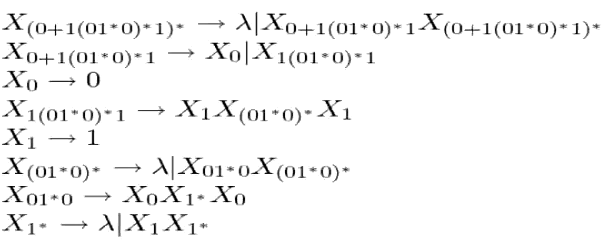
\includegraphics{t3-2.png}

& Para todo lenguaje regular, existe una gramática que lo genera. Es decir, la clase de los lenguajes regulares está incluida dentro de la clase de los lenguajes incontextuales.

& Hay una manera más sencilla de obtener una gramática a partir de un autómata que es más directa.

& Este es el autómata de los múltiples de 3.

\ \begin{tikzpicture}[->,>=stealth',shorten >=1pt,auto,node distance=2.8cm,semithick]

\node[initial, accepting, state] (A)  {$0$};
\node[state] (B) [right of=A] {$1$};
\node[state] (C) [right of=B] {$2$};


  \path (A) edge [loop above] node {$0$} (A)
        (C) edge [loop right] node {$1$} (C)
        (A) edge [bend left] node {$1$} (B)
        (B) edge [bend left] node {$1$} (A)
        (B) edge [bend left] node {$0$} (C)
        (C) edge [bend left] node {$0$} (B);
\end{tikzpicture}


& Y esta es la gramática que obtenemos a partir de él:

\Deactivate
$$\begin{array}{lcl}
X_0 &\to& \lambda | 0X_0 | 1X_1\\
X_1 &\to& 0X_2 | 1X_0\\
X_2 &\to& 0X_1 | 1X_2\end{array}$$
\Activate


& Tenemos una variable de la gramática para cada estado del autómata ($X_0$, $X_1$ y $X_2$). El objetivo de $X_0$ es generar todas las palabras que nos llevan a estado aceptador empezando la ejecución desde el estado 0. Y lo mismo para $X_1$ y $X_2$.

& Las palabras que nos llevan a estado aceptador desde el estado $0$ o bien son la palabra vacía (porque el estado es aceptador), o bien empiezan por $0$ y vienen seguidas de una palabra que nos lleva desde el estado $0$ al estado aceptador, o bien empiezan por $1$ y vienen seguidas de una palabra que nos lleva desde el estado $1$ al estado aceptador. Lo mismo sucede para $X_1$ y $X_2$. En estos dos últimos casos, no aceptamos la palabra vacía porque no son estados aceptadores.

& Por la construcción de la gramática, resulta obvio que genera el lenguaje reconocido por el autómata. Un argumento inductivo nos permitiría demostrarlo. De hecho, esta gramática simula el autómata.

& Considérese la ejecución aceptadora $$q_0 10101 = q_1 0101 = q_2 101 = q_2 01 = q_1 1 = q_0.$$

& Mediante la derivación $$X_0 \to_G 1X_1 \to_G 10X_2 \to_G 101X_2 \to_G 1010X_1 \to_G 10101X_0 \to_G 10101,$$ la gramática genera la misma palabra a base de ir recordando el estado en el que se encuentra el autómata con la palabra leída hasta el momento. Las $\lambda$-producciones, que tan solo aparecen en las variables de estados aceptadores, nos permiten terminar la derivación.

& Las gramáticas tales que cada parte derecha de regla tiene como mucho una variable, y donde esta aparece cuanto más a la derecha posible se denominan gramáticas lineales por la derecha, o gramáticas regulares por la derecha. Este tipo de gramáticas siempre generan lenguajes regulares.

& Existe una transformación similar de autómatas en gramáticas lineales por la izquierda, también llamadas gramáticas regulares por la izquierda. Estas se definen de manera análoga.
\end{easylist}
\section{Gramáticas incontextuales}

% \Deactivate
% $$\begin{array}{lcl}
% X_0 &\to& \lambda | 0X_0 | 1X_1\\
% X_1 &\to& 0X_2 | 1X_0\\
% X_2 &\to& 0X_1 | 1X_2\end{array}$$
% \Activate

\subsection{Gramáticas incontextuales}
\begin{easylist}[itemize]
& Una gramática incontextual (CFG de \textit{Context Free Grammar}) $G$ es un conjunto de reglas de reemplazo donde las partes izquierda son palabras de longitud 1. A las reglas también se les suele llamar \textit{producciones}.

\Deactivate
$$\begin{array}{lcl}
S &\to& aS\\
S &\to& X\\
X &\to& aXb\\
X &\to& \lambda
\end{array}$$
\Activate

& A todo símbolo que aparezca a la izquierda de alguna regla lo llamaremos \textit{variable} o \textit{no terminal}. Generalmente, los denotamos con letras mayúsculas.

& Al resto de símbolos los llamamos \textit{terminales} y, normalmente, los notamos con letras minúsculas.

& En este caso, $S$ y $X$ son variables mientras que $a$ y $b$ son terminales.

& Usualmente la lista de reglas se representa de forma comprimida agrupando las partes derecha de regla de cada variable. Por ejemplo: 

\Deactivate
$$\begin{array}{lcl}
S &\to& aS\; | \; X\\
X &\to& aXb \; | \; \lambda
\end{array}$$
\Activate

& En una gramática, siempre se distingue una variable inicial, llamada \textit{símbolo inicial} (en este caso, $S$) que, por defecto, es la primera que aparece.

& Las palabras generadas por la gramática son las formadas por terminales y que sean alcanzables desde el símbolo inicial.

& Ejemplo de derivación de $G$: vamos reemplazando los símbolos subrayados por los resultados de las reglas de reemplazo. Así: $\underline{S} \to_G a\underline{S} \to_G a\underline{X} \to_G aa\underline{X}b \to_G aab$. Esta palabra ya es terminal. Así pues, $aab$ es una palabra generable por la gramática $G$.

& Una derivación se puede representar, también, en forma de árbol. En la raíz situamos el símbolo inicial. Vamos colgando en cada sustitución los cambios que hacemos.

\ \begin{tikzpicture}[level distance = 10mm, sibling distance = 10mm]
\node {$S$}
child {node {$a$}}
child {
    node {$S$}
    child {
        node {$X$}
        child {node{$a$}}
        child {
                node{$X$}
                child {node{$\lambda$}}
            }
        child {node{$b$}}
    }
};
\end{tikzpicture}

& La palabra generada será la concatenación de todas las hojas: $aa\lambda b = aab$. A este tipo de árbol se le llama \textit{árbol sintáctico}.

& A veces, las CFG se representan más formalmente con una tupla $G = \langle V, \Sigma, \delta, S\rangle$ que contiene el alfabeto de variables o no terminales, el alfabeto de  símbolos no terminales, el conjunto de reglas y cuál de las variables es el símbolo inicial.

& En el ejemplo anterior, $$G = \langle \{S, X\}, \{a, b\}, \{S \to aS, S\to X, X \to aXb, X\to\lambda\}, S\rangle.$$

& El lenguaje generado por una gramática se define como el conjunto de palabras formadas por símbolos terminales y generables desde el símbolo inicial: $\mathcal L (G) = \{w\in \Sigma^* \colon S\to_G^* w\}$.

& El lenguaje generado por una variable concreta de la gramática es el conjunto de palabras terminales generables desde esa variable: $\mathcal L(G, X) = \{w \in \Sigma^* \colon X\to_G ^* w\}$.

& El ejemplo anterior genera el lenguaje $\mathcal L(G) = \{a^nb^m\ \colon n \geq m\}$. Esto es, las palabras con unas cuantas $a$s seguidas de unas cuantas $b$s donde hay más o igual $a$s que $b$s.

& A un lenguaje se le llama lenguaje incontextual, o CFL si existe una gramática que lo genera: $L \in \textrm{CFL} \iff\exists G \in \textrm{CFG} \colon \mathcal L(G) = L$.

& Existen algoritmos para comprobar si una palabra es generable por una gramática y, en caso afirmativo, construye un árbol de generación o sintáctico.

& El árbol es útil pues nos estructura una palabra de entrada que, inicialmente, no era más que una secuencia de símbolos. Por ejemplo, relación entre lenguajes de programación y compiladores.

& Una gramática alternativa equivalente a la anterior es $S \to aS \;|\; aSb \;|\; \lambda$. En este caso, hay un solo no terminal. Desde $S$ podemos escoger si añadimos una $a$ o añadimos una $a$ y una $b$ al mismo tiempo.

& Esta gramática tiene un problema: tiene árboles de derivación diferentes para una misma palabra $aab$.

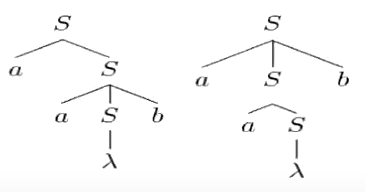
\includegraphics{t4-2.png}

& Cuando una gramática permite más de un árbol de derivación para alguna palabra, decimos que es \textit{ambigua}.

& Otra gramática ambigua es:

\Deactivate
$$\begin{array}{lcl}
E &\to& E + E \; | \; E - E \; | \; N\\
N &\to& ND \; | \; D\\
D &\to& 0|1|2|3|4|5|6|7|8|9
\end{array}$$
\Activate

& Una expresión puede ser suma de expresiones o resta de subexpresiones o un número. Un número puede ser uno o más dígitos.

& Podemos generar la palabra $7 - 4 + 2$. \textit{A priori}, la palabra no significa nada.

& Hay dos árboles de derivación diferentes para esta palabra.

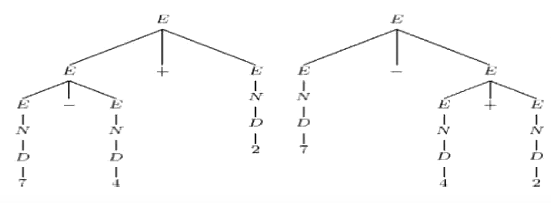
\includegraphics{t4-3.png}

& Ambos árboles son útiles para comprobar que nuestra palabra de entrada pertenece a la gramática. Sin embargo, los árboles de derivación se pueden usar luego para dar significado a las palabras que generan.

& En el caso de la izquierda, resulta que primero hay que restar $7$ y $4$ y luego la suma de $2$ y la subexpresión anterior. En el otro, es al revés.

& En el supuesto caso que usemos un generador automático de árboles sintácticos a partir de una gramática y una entrada, si la gramática es ambigua, corremos el riesgo de que los árboles obtenidos no se correspondan a la interpretación que queremos dar a las entradas. Por ese motivo, el motivo de ambigüedad es importante y conviene tenerlo en cuenta al usar reconocedores automáticos.

& Una gramática equivalente a la anterior y no ambigua es
\Deactivate
$$\begin{array}{lcl}
E &\to& N + E \; | \; N - E \; | \; N\\
N &\to& ND \; | \; D\\
D &\to& 0|1|2|3|4|5|6|7|8|9
\end{array}$$
\Activate

& Nótese que estamos obligados a escoger la primera regla si el primer operador es suma, y la segunda regla si el primer operador es resta. De este modo, la palabra que queremos generar determina de forma unívoca la regla a utilizar en cada nodo.

\end{easylist}








\subsection{Operaciones sobre gramáticas incontextuales}
Cuando operamos dos lenguajes incontextuales con ciertas operaciones conocidas, el resultado es, nuevamente, un lenguaje incontextual.


\subsubsection{Unión}

\begin{easylist}[itemize]
& Los lenguajes incontextuales son cerrados por unión: si hay gramáticas para $L_1$ y $L_2$, entonces $L_1, L_2 \in \textrm{CFL} \implies L_1 \cup L_2 \in \textrm{CFL}$.

& Sean $G_1 = \langle V_1, \Sigma_1, \delta_1, S_1\rangle$ y $G_2 = \langle V_2, \Sigma_2, \delta_2, S_2\rangle$ gramáticas tales que reconocen los lenguajes $L_1$ y $L_2$; esto es, $\mathcal L(G_1) = L_1$ y $\mathcal L(G_2) = L_2$.\footnote{También hemos de suponer que $V_1 \cap V_2 = \varnothing$. Esto es, que no comparten variables libres. Pero esto no conlleva una pérdida de generalidad, pues, sin ningún problema podemos renombrar las variables en una de las gramáticas de manera que aquella gramática siga generando el mismo lenguaje.}

& La unión de $L_1$ y $L_2$ es, y notado abusivamente, $L_1 \cup L_2 = \langle V_1 \cup V_2 \cup \{S\}, \Sigma_1 \cup \Sigma_2, \delta_1 \cup \delta_2 \cup \{S \to S_1 | S_2\}, S \rangle$.

& Esto es, añadimos una nueva regla a partir de $S$: $S_1$ o $S_2$.

& Por tanto, $\mathcal L(G_1 \cup G_2) = \mathcal L(G_1) \cup \mathcal(G_2) = L_1 \cup L_2$.
\end{easylist}


\subsubsection{Intersección}
\begin{easylist}[itemize]
& Los lenguajes \textit{no} están cerrados por interseccción: esto es, que $L_1, L_2 \in \textrm{CFL}$ no implica $ L_1 \cap L_2 \in \textrm{CFL}$.

& Por ejemplo, no es difícil encontrar gramáticas para los lenguajes $\{a^nb^nc^m \colon n,m \geq 0\}$ y $\{a^nb^mc^m \colon n,m\}$ (ambos $\in \textrm{CFL}$); pero su lenguaje intersección, $\{a^nb^nc^n \colon n \geq 0\}$ no es incontextual, como veremos en otra sección.

\end{easylist}

\subsubsection{Complementario}

\begin{easylist}[itemize]
& Los lenguajes tampoco están cerrados por complementario. Si lo estuviesen, como $L_1 \cap L_2 = \overline{\overline{L_1} \cup \overline{L_2}}$, entonces la intersección también sería una operación cerrada para lenguajes incontextuales, cosa que hemos visto que no es así.
\end{easylist}


\subsubsection{Concatenación}

\begin{easylist}[itemize]
& Los lenguajes incontextuales están cerrados por concatenación: $L_1, L_2 \in \textrm{CFL} \implies L_1 \cdot L_2 \in \textrm{CFL}$.

& Esto es, sean $G_1 = \langle V_1, \Sigma_1, \delta_1, S_1\rangle$ y $G_2 = \langle V_2, \Sigma_2, \delta_2, S_2\rangle$ gramáticas tales que reconocen los lenguajes $L_1$ y $L_2$; esto es, $\mathcal(G_1) = L_1$ y $\mathcal (G_2) = L_2$, con $V_1 \cap V_2 = \varnothing$.

& $G_1 \cdot G_2 = \langle V_1 \cup V_2 \cup \{S\}, \Sigma_1 \cup \Sigma_2, \delta_1 \cup \delta_2 \cup \{S \to S_1S_2\}, S \rangle$. La diferencia está en que, ahora, desde el símbolo inicial de la gramática generamos la concatenación de $S_1$ con $S_2$.

& De esta manera, desde $S$ podemos generar todas las palabras que se forman al concatenar una palabra de $L_1$ con otra de $L_2$.

& Así pues, queda claro que generamos el lenguaje concatenación de $L_1$ y $L_2$: $\mathcal L(G_1 \cdot G_2) = \mathcal L(G_1) \cdot \mathcal L(G_2) = L_1 \cdot L_2$.
\end{easylist}

\subsubsection{Estrella}
\begin{easylist}[itemize]
& Los lenguajes incontextuales están cerrados por la operación estrella. Es decir: si $L \in \textrm{CFL}$, entonces $L^* \in \textrm{CFL}$.

& Si $G = \langle V, \Sigma, \delta, S\rangle$ tal que $\mathcal L(G) = L$, entonces $G^* = \langle V \cup \{S'\}, \Sigma, \delta \cup \{S' \to S'S|\lambda\}, S'\}$ cumple $\mathcal L(G^*) = \mathcal L (G)^* = L ^*$.

& Añadimos una regla tal que, desde $S'$, generamos $0$ o más $S'$s; esto es, $0$ o más palabras de $S$.
\end{easylist}

\subsubsection{Reverso}
\begin{easylist}[itemize]
& Los lenguajes incontextuales están cerrados por reverso. Es decir: si $L \in \textrm{CFL}$, entonces $L^R \in \textrm{CFL}$.

& La gramática reverso se obtiene simplemente manteniendo las mismas reglas pero haciendo el reverso de sus partes derecha.

& $G^R = \langle V, \Sigma, \{X \to u^R \colon (X \to u) \in \delta\}, S'\rangle$. Esto es, $\mathcal L(G^R) = \mathcal L(G)^R = L^R$.\footnote{Mirad \url{https://youtu.be/rHOyFDCOKbs} a partir del minuto 5:26 para una justificación exhaustiva de esta propiedad.}
\end{easylist}







\subsection{Depuración de gramáticas (1)}
\begin{easylist}[itemize]
\end{easylist}

\textit{Falta redactarlo}





\subsection{Depuración de gramáticas (2)}
\begin{easylist}[itemize]
\end{easylist}


\textit{Falta redactarlo}




\subsection{Depuración de gramáticas (3)}
\begin{easylist}[itemize]
\end{easylist}

\textit{Falta redactarlo}
\section{No regularidad}
\subsection{No regularidad (1)}
\begin{easylist}[itemize]
& En esta sección justificaremos que ciertos lenguajes no son regulares o incontextuales. A este tipo de resultados se les llama, a veces, resultados negativos, pues muestran las limitaciones de expresividad de un cierto formalismo.

& Vamos a ver el lenguaje $\{a^n b^n \colon n \geq 0\}$ no es regular ($\notin \mathrm{Reg}$). Nótese que este contiene exactamente a las palabras que empiezan por un número de $a$s seguidas de el mismo número de $b$s. Por simplicidad, lo llamaremos el lenguaje $a^n b^n$.

& Intuitivamente, ya parece ser no regular, pues los autómatas tienen un número finito de estados. Y no serán suficientes para recordar todas las $a$s necesarias hasta el momento, cosa necesaria para comprobar luego si tenemos tantas $b$s como $a$s.

& Procedemos, por reducción al absurdo, que $\{a^n b^n \colon n \geq 0\} \in \mathrm{Reg}$. Entonces, existe un DFA $A = \langle Q, \Sigma, \delta, q_0, F\rangle$ que lo reconoce. Esto es, tal que $\mathcal L(A) = \{a^n b^n\}$. Sea $N = |Q|$ (el número de estados de $A$). Si ejecutamos el autómata con entrada $a^N$, pasamos por los estados $q_0$, $q_0a$, $q_0a^2$, $\dots$, $q_0 a^N$. En total, hay $N + 1$ estados; como $N + 1 > N = |Q|$, entonces, necesariamente hay dos repetidos. Esto es, existen $0 \leq i < j \leq N$ tales que $q_0 a^i = q_0 a^j$. Pero entonces, $q_0 a^i b^i = q_0 a ^j b ^i$. Este estado tiene que ser aceptador porque $a^i b ^i \in \{a^n b^n\}$. Pero hemos visto que $a ^j b^i \notin \{a^n b^n\}$ (no es aceptador). Contradicción.

& El lenguaje $a^n b^n$ es incontextual, pues lo genera la gramática $S \to aSb | \lambda$.

& Esto justifica que la inclusión de los lenguajes regulares dentro de los lenguajes incontextuales es estricta: $\mathrm{Reg} \subsetneq \mathrm{CFL}$.

& La técnica que acabamos de ver suele funcionar para demostrar la no regularidad de muchos lenguajes. Sin embargo, a veces podremos encontrar una demostración mucho más rápida aprovechando que $a^n b^n $ no es regular.

& Por ejemplo, queremos demostrar que $\overline{\{a^n b^n \colon n \geq 0\}}$ no es regular.

& Procedemos por reducción al absurdo suponiendo que lo es. Como los lenguajes regulares están cerrados por complementario, deducimos que el complementario de este lenguaje también es regular. Pero este complementario es precisamente $a^n b^n $, que hemos demostrado anteriormente que no es regular. Contradicción.

& Lo anterior también se aplica para la unión, la intersección, concatenación, estrella, reverso, morfismo directo y morfismo inverso. Procediendo de forma análoga a como lo hemos hecho aquí, podemos demostrar la no regularidad aprovechándonos de las propiedades anteriores.

& Ahora veremos que $a^n b^n c^n \notin \mathrm{CFL}$ (no es incontextual).

& Procedemos por reducción al absurdo suponiendo que sí lo es. Entonces, existe una gramática incontextual CFG $G = \langle V, \Sigma, \delta, S \rangle$ tal que $\mathcal L(G) = \{a^n b^n c^n\}$ que lo genera. Sin pérdida de generalidad, podemos suponer que $G$ está en forma normal de Chomsky CNF. Sea $N = |V|$ el número de variables de $G$.

& Consideramos la palabra $a^{2^N} b^{2^N} c^{2^N}$, que es del lenguaje, y, por tanto, existe un árbol de derivación de la misma con las reglas de $G$.

& Nótese que el número de hojas de este árbol es mayor a $2^N$. Además, como la gramática está en forma normal de Chomsky, todos los nodos internos tienen aridad como mucho $2$. De hecho, todos tienen aridad $2$ excepto aquellos que quedan por encima de las hojas. Así pues, no es difícil inferir que el árbol tiene altura mayor que $ N$. Ya que los árboles con altura $\leq N$ y aridad como mucho $2$ tienen, a lo sumo, $2^N$ hojas.

& En consecuencia, en el árbol existirá un camino de longitud $N$ desde la raíz hasta una de las hojas. Dado que $N$ es el número de variables distintas de $G$, podemos concluir que existirá un camino desde la raíz hasta una hoja en el que se repita la ocurrencia de una variable, digamos, $x$. Por tanto, existe una derivación de la forma  $S \to_G^* w_1 X w_5 \to_G^* w_1 w_2 X w_4 w_5 \to_G ^* w_1 w_2 w_3w_4w_5 = a^{2^N} b^{2^N} c^{2^N}$ y, en ella, habrá una derivación desde $X$ así: $X \to _G ^+ w_2 X w_4$.

& Como $G$ está en CNF, no hay ni $\lambda$-producciones ni producciones unarias en $G$, de modo que, en la subderivación desde $X$ se genera algún símbolo de más.

& De ello se infiere que, o bien $w_2$, o bien $w_4$, tiene tamaño mayor a 0.

& Por otro lado, podemos modificar la derivación desde $S$ así: $S \to_G^* w_1 X w_5 \to_G^* w_1 w_2 X w_4 w_5 \to_G ^* w_1 w_2 w_2 X w_4 w_4 w_5 \to_G ^* w_1w_2w_2 w_3 w_4 w_4 w_5$. Hemos replicado la subderivación desde $X$ y, de este modo, alcanzamos esta palabra $w$.

& Como es una palabra terminal generable desde el símbolo inicial, tiene que ser del lenguaje. Esto es, $w = w_1 w_2 w_2 w_3 w_4 w_4 w_5 \in \{a^n b^n c^n\}$.

& De ello podemos inferir que $w_2, w_4 \in (a^* + b^* + c^*)$. Esto es, están formadas por un único símbolo.

& Resumiendo, $w$ tiene algún símbolo de más respecto la palabra inicial del lenguaje porque, o bien $w_2$ o $w_4$ es vacío. Pero, o bien no añade $a$s, o bien no añade $b$s, o bien no añade $c$s. Como consecuencia, no puede tener el mismo número de $a$s, $b$s y $c$s. Pero habíamos supuesto que sí que era del lenguaje. Contradicción.
\end{easylist}





\subsection{No regularidad (2)}
Se trata de una demostración análoga a la anterior.

Consultad \url{youtu.be/0QkKBOTE4a4} para más información.

\begin{easylist}[itemize]
\end{easylist}
\section{Máquinas de Turing}
\subsection{Máquinas de Turing (1)}
\begin{easylist}[itemize]
& Las máquinas de Turing son un mecanismo de cómputo muy sencillo de definir. Sin embargo, son tan potentes como cualquiera de los lenguajes de programación que usamos hoy en día. Por ser de demasiado bajo nivel, no resultan prácticas para programar. Su utilidad es en el sentido contrario: gracias a ser tan simples, resulta más fácil demostrar que algo no se puede resolver con ellas. Y gracias a su equivalencia a los lenguajes de programación, facilitan demostrar que un cierto problema no se puede resolver con ningún lenguaje de programación.

& Más adelante, definiremos el concepto de lenguaje decidible como aquél reconocible por una máquina de Turing de parada segura.

& Una de las particularidades de las máquinas de Turing es que tienen un dispositivo de memoria de tamaño infinito. Eso puede parecer no razonable si queremos usarlas para representar qué cosas podemos decidir o computar y cuáles no con nuestras máquinas reales.

& Las máquinas reales tienen memoria finita. Por tanto, esencialmente, se pueden describir mediante un autómata finito determinista. Cada una de sus configuraciones estará representada por un estado, y un cambio de configuración corresponde a una transición entre estados. Aún así, hay razones que llevan a preferir no definir los lenguajes decidibles como aquellos decidibles como aquellos reconocibles por autómatas finitos deterministas. 

& En primer lugar, nótese queM en una máquina con, al menos 1 GB de memoria tendrá, al menos, $2^{23}$ bits; y, por tanto, al menos, tendrá $2^{2^{23}}$ configuraciones posibles (estados). Ese número es mucho mayor que el número de átomos en el universo (sobre $10^{77}$).

& Por tanto, no tiene sentido describir el comportamiento de nuestras máquinas como el de un mecanismo que no es transportable a la vida real. Además, si definimos \textit{lenguaje decidible} como aquel reconocible mediante un DFA, sacaremos conclusiones que no nos parecen razonables.

& Por ejemplo, concluiríamos que el lenguaje $\{a^n b^n\}$ no es decidible. Sin embargo, todo informático afirmará que sabe escribir un programa que decida si tenemos tantas $a$s como $b$s en una cadena de entrada. Por estos motivos, y porque la memoria disponible en las máquinas que usamos aumenta, se suele considerar como algoritmo a la combinación de un control de ejecución finito y memoria infinita.

& Vamos a ver más en profundidad las máquinas de Turing. Estas tienen un grafo de estados y transiciones como en los DFA. Pero, además, tienen lo que llamaremos \textit{cinta}, que es una palabra con infinitas posiciones.

& Para que el autómata maneje este dispositivo, en todo momento hay un apuntador a una de las posiciones de la cinta que llamaremos \textit{cabezal}.

& Las transiciones del autómata tendrán una condición para su ejecución que será que el símbolo guardado en la posición apuntada por el cabezal tenga que ser uno concreto.

& Además, cada transición tendrá una acción indicando qué símbolo hay que escribir en la posición apuntada por el cabezal, y si queremos mover el cabezal a derecha, izquierda o dejarlo quieto.

& Inicialmente, la máquina se encuentra en el estado incial, el cabezal apunta a la posición $1$, y en la cinta se halla la palabra de entrada de la máquina, empezando por la posición $1$.

& En la posición $0$ se halla un símbolo especial que no forma parte del alfabeto de entrada, y que llamaremos \textit{símbolo de marca de inicio} ($\vartriangleright$). Si lo gestionamos bien, siempre que veamos este símbolo, sabremos que nos encontramos lo más a la izquierda posible de la cinta.

& Después del último símbolo de la entrada, nos aparece un símbolo que llamaremos \textit{símbolo de blanco} o, simplemente, \textit{blanco} (\textblank). A partir de ese punto, todos los símbolos que aparecen son blancos.

& La máquina empezará su ejecución. Se irán ejecutando transiciones cuando se cumplan sus condiciones; como consecuencia, el cabezal se irá desplazando y, a su vez, se modificará el contenido de la cinta.

& Los símbolos que se escriban pueden ser del propio alfabeto de entrada pero también pueden no serlo. La palabra de entrada será aceptada si, finalmente, llegamos al único estado aceptador que tendrá la máquina y que marcaremos como en los DFA.

& Vamos a ver un ejemplo más concreto. Queremos construir una máquina de Turing que reconozca el lenguaje $\{w \# w \colon w \in \{0, 1\}^*\}$.

& Si la palabra efectivamente es del lenguaje, entonces la cinta tendrá este aspecto: $\vartriangleright\; 0\;1\;1 \cdots \#\; 0\;1\;1\cdots \blanco\; \blanco\cdots$, y el cabezal apuntará al primer símbolo. 

& Nos interesa ir comprobando que los símbolos de las correspondientes posiciones coinciden. Lo que haremos será recordar, mediante los estados, qué símbolo se encuentra al principio; nos moveremos hasta el principio de la segunda parte y veremos si también se halla el mismo símbolo al principio. Y, así, sucesivamente con los siguientes símbolos.

& Pero para que la máquina pueda saber qué parte de las palabras ha sido ya comprobada, iremos sustituyendo los símbolos ya tratados por símbolos nuevos a modo de marca. Por tanto, lo que haremos es: leer el primer $0$, marcarlo como $0'$ y movernos a la derecha hasta saltar el separador y recordando que hemos visto un $0$. Al ver el otro $0$, lo marcamos también y volvemos atrás saltándanos el separador hasta encontrar nuevamente la marca inicial.

& Ahora leemos un $1$, lo marcamos y vamos hacia la derecha saltándonos el separador y las marcas que encontremos, recordando que hemos visto un 1. Al comprobar que aquí hay un $1$, lo marcamos y volvemos atrás, y así, sucesivamente, hasta que hayamos comprobado que ambas palabras son iguales.

& Aquí tenemos la representación de la máquina de Turing.

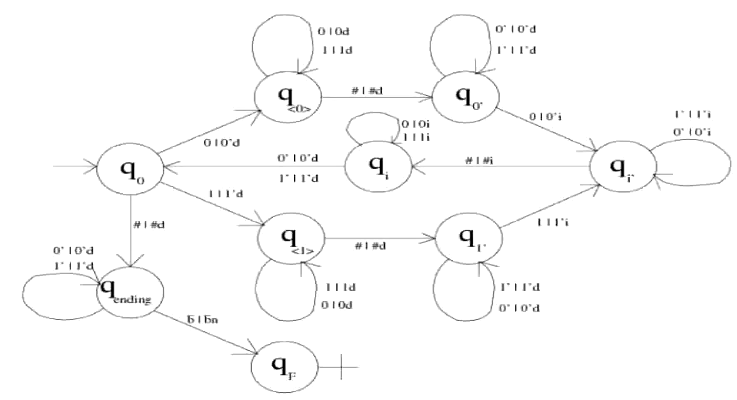
\includegraphics[width=0.8\textwidth]{t7-1.png}

& El estado inicial es $q_0$; el aceptador es $q_F$.

& Las transiciones están etiquetadas con:
&& Por un lado, el símbolo de condición para que se ejecute que es el símbolo que esperamos ver en la cinta.
&& Por otro lado, la acción que consta de qué símbolo se escribe en la cinta y si movemos el cabezal a la derecha, en este caso, o a la izquierda o no lo movemos ($d$, $i$, $n$).

& Desde el estado inicial, si leemos un $0$, lo marcamos con $0'$ y vamos hacia la derecha. Este estado $q_{<0>}$ recuerda que hemos visto un $0$, y va saltando (el bucle) símbolos hasta que lee el símbolo separador; después, va saltando símbolos marcados esperando ver, finalmente un $0$. Ese $0$ se marca y se inicia el proceso de retorno hacia la izquierda. Nos saltaremos los símbolos marcados a la derecha del separador ($q_{i'}$), luego el símbolo separador, y, después, los no marcados de la izquierda ($q_i$) hasta que encontremos, nuevamente, el símbolo marcado. En ese momento (de $q_i$ a $q_0$), nos movemos una posición a la derecha y reiniciamos el proceso.

& El caso en que veamos un $1$ desde $q_0$ se trata de forma análoga.

& Cuando vemos el separador desde $q_0$, señal de que ya hemos marcado todos los símbolos a la izquierda del separador. Para terminar de asegurarnos de que la palabra es del lenguaje; bastará con que comprobemos que todos los símbolos a la derecha del separador también han sido marcados. Esto es lo que hace $q_\text{ending}$. Cuando vemos el símbolo de blanco, saltamos a estado aceptador ($q_F$).

\end{easylist}





\subsection{Máquinas de Turing (2)}
\begin{easylist}[itemize]
& En esta sección vemos una formalización de las máquinas de Turing y definimos lenguajes decidibles, lenguajes semidecidibles y funciones computables.

& Las máquinas de Turing se pueden representar como una tupla con los siguientes elementos: $\langle Q, \Sigma, \Gamma, \delta, q_0, q_F\rangle$. Donde $Q$ es el conjunto de estados, $\Sigma$ es el alfabeto de las palabras de entrada, $\Sigma$ es el alfabeto de cinta, $\delta$ la función de transición, $q_0$ es el estado inicial y $q_F$ es el estado aceptador.

& El alfabeto de cinta siempre contiene al alfabeto de entrada y, adicionalmente, al símbolo de inicio de cinta y al símbolo de blanco. Estos dos no pertenecen al conjunto de entrada; por eso ponemos unión disjunta: $\Sigma \uplus \{\vartriangleright, \blanco \} \subseteq \Gamma$. Por supuesto, el alfabeto de cinta puede contener más de símbolos a parte de todos estos.

& La función de transición nos dice para cada estado que no sea el aceptador y cada símbolo de cinta, a qué otro estado vamos a parar, qué nuevo símbolo se escribe en la cinta y hacia dónde movemos el cabezal con opciones: \textit{izquierda}, \textit{derecha} y \textit{no mover}. Esto es: $\delta \colon Q - \{q_F\} \times \Gamma \to Q \times \Gamma \times \{i, d, n\}$.

& La función de transición es parcial: es decir, pueden no estar definida para todos los estados y símbolos posibles.

& También es posible considerar el caso no determinista. En tal caso, la función de transición ya no sería necesariamente una función, sino un subconjunto del producto cartesiano de todos los conjuntos anteriores.

& Una configuración de una máquina de Turing es un estado global en que esta se puede encontrar en algún momento. La configuración describe no sólo al estado, sino también al contenido de la cinta y a la posición del cabezal.

& El contenido de la cinta es, en realidad, infinito. Sin embargo, tan solo un número finito de sus posiciones contendrán símbolos que no sean blancos. Ya que, en un tiempo finito de ejecución, tan solo se han podido modificar un número finito de posiciones. Por ese motivo, para describir el contenido de la cinta, basta con una palabra finita.

& Usualmente, describimos una configuración del modo $w_1qw_2$. El contenido de la cinta antes del cabezal es $w_1$, el estado en que se encuentra la máquina es $q$, y $w_2$ es el contenido de la cinta desde el cabezal en adelante. En particular, el primer símbolo de $w_2$ es el apuntado por el cabezal. Se asume que más allá de $w_2$ hay blancos. Por ese motivo, esta configuración se considera equivalente a $w_1 q w_2 \blanco \blanco \blanco$ (todos los blancos que queramos).

& La función de transición $\delta$ también se puede representar mediante un sistema de reescritura con reglas que se aplican sobre configuraciones.

& Nótese que una transición de desplazamiento hacia la derecha se puede representar mediante la regla $qa \to bq'$. La regla se aplica sobre una configuración si el estado es $q$ y el símbolo apuntado por el cabezal es $a$. Reemplaza localmente el símbolo $a$ por $b$ y mueve el cabezal hacia la derecha, y cambia el estado a $q'$.

& De manera similar, si la transición no desplaza el cabezal, esta regla nos permite representarla: $qa \to q'b$.

& En el caso de transiciones que desplazan el cabezal hacia la izquierda, la situación se complica ligeramente, porque la regla necesita saber qué símbolos se encuentran a la izquierda del cabezal. Por ese motivo, transiciones de este estilo se representan mediante tantas reglas como símbolos tiene el alfabeto de cinta. En esta descripción, estamos asumiendo que $a_1$ hasta $a_n$ son los símbolos del alfabeto de cinta: $a_1 q a \to q' a_1 b, \dots, a_n q a \to q' a_n b$.

& Definimos el lenguaje aceptado o reconocido por una máquina de Turing como el conjunto de palabras que nos llevan a estado aceptador. Esto es: $\mathcal L(M) = \{w \in \Sigma^* \colon \exists w_1, w_2 \in \Gamma^*, n \in \mathbb N \colon \vartriangleright w  \blanco^n \to_\delta ^* w_1 q_F w_2\}$. Más concretamente, son aquellas palabras sobre el alfabeto de entrada tales que, añadiendo el símbolo de inicio de cinta a su izquierda y un número suficiente de blancos a su derecha pueden acceder por reescritura de la función de transición hasta una configuración cuya estado sea aceptador ($w_1 q_F w_2$).

& Definimos la función computada por una máquina de Turing del siguiente modo. Un elemento $x$ tiene como imagen $y$ si, teniendo $x$ como entrada, la máquina llega a estado aceptador dejando $y$ en la cinta. Más concretamente, si $x$ e $y$ se forman sobre el alfabeto de entrada y, además, tras añadir el símbolo de inicio de cinta a la izquierda de $x$ y suficientes blancos a su derecha accedemos a una configuración con estado aceptador y que contenga $y$ entre el primer y segundo símbolo fuera del alfabeto de entrada ($\alpha_1 y \alpha_2 w')$, entonces decimos que $y$ es la imagen de $x$ por la función computable por la máquina.

& Fijaos que, mediante la aplicación de la regla adicional $q_F \to \Gamma$, estamos borrando el estado aceptador de la configuración para poder hablar únicamente del contenido de la cinta. Es decir: $\varphi_M (x) = y$ es equivalente a $x,y\in\Sigma^*$ y, además, existen $\alpha_1, \alpha_2 \in (\Gamma - \Sigma), w' \in \Gamma^*, n \in \mathbb N$ tales que $\vartriangleright x  \blanco^n \to_{\delta \cup \{q_F \to \lambda \}} \alpha_1 y \alpha_2w'$.

& No es difícil convencerse de que el dominio de la función computada por la máquina $M$ es justamente el lenguaje reconocido por $M$: $\textrm{Dom}(\varphi_M) = \mathcal L (M)$.

& De este modo, denotamos que la imagen de $x$ por $\varphi_M$ está definida. Es decir, que existe una $y$ que es su imagen: $\varphi_M (x) \downarrow \equiv \exists y \colon \varphi_M (x) = y \equiv x \in \mathcal L (M)$.

& Decimos que una configuración es terminal si no se le puede aplicar ninguna regla: $\nexists w' \in \Gamma^* \colon w  \blanco \to _\delta w'$.

& De este modo, denotamos que la máquina $M$ con entrada $x$ termina su ejecución en algún momento: $M(x) \downarrow$. Es decir, que existe $n \in \mathbb N$ y una configuración terminal $w$ tal que $\vartriangleright x  \blanco^n  \to _\delta ^* w$.

& Nótese que toda configuración aceptadora es terminal por tanto, si la imagen de $x$ está definida, entonces la máquina para con entrada $x$: $\varphi_M (X) \downarrow \implies M(x) \downarrow$. Sin embargo, la implicación contraria no es necesariamente cierta, ya que puede haber configuraciones terminales que no sean aceptadoras. Símplemente puede ocurrir que no se pueda aplicar ninguna regla por no haber más transiciones definidas.

& En el caso en que $\varphi_M(x)$ esté definida, entonces, por $M(x)$ también denotamos $\varphi(x)$.

& Definimos un lenguaje como decidible si existe una máquina de Turing que lo reconoce y que para con toda entrada. En tal caso, decimos que la máquina decide el lenguaje. Esto es, $L$ es decidible ($L \in \textrm{Dec}$) si existe una máquina de Turing $M$ tal que $\mathcal L(M) = L$ y $M$ para con toda entrada.

& Definimos un lenguaje como semidecidible o recursivamente numerable si existe una máquina de Turing que lo reconoce. En tal caso, decimos que la máquina semidecide el lenguaje. Así pues, semidecidir y reconocer son palabras sinónimas. Esta máquina puede no parar con aquellas entradas que no sean del lenguaje. En definitiva: $L$ es semidecidible ($L \in \textrm{semi-Dec}$) si $\exists M \in \textrm{TM}$ tal que $\mathcal L(M) = L$.

& Definimos una función como computable si existe una máquina que la computa. En tal caso, decimos que esa máquina es una implementación de la función o que computa la función: $f\colon \Sigma^* \to \Sigma^*$ es computable si y solo si existe una máquina de Turing $M$ tal que $\varphi_M = f$. Nótese que $f$ no necesariamente debe ser total, y que otra definición alternativa a computabilidad es: $f$ es computable si y solo si para toda entrada del dominio $w$, $M(w) \downarrow$ en $q_F$ de manera que $M(w) = f(w)$. Cabe notar que, para las entradas $w$ que no son del dominio, puede pasar que $M(w) \uparrow$ o bien $M(w) \downarrow$ en estado $q_F$. Solo nos importan las palabras del dominio


\end{easylist}

\section{Decibilidad, semidecibilidad y computabilidad}
\subsection{Equivalencia entre TM y programas}
\subsubsection{\textit{k}-máquina de Turing}
\begin{easylist}[itemize]
& En esta sección veremos que las TM son tan expresivas como cualquiera de los lenguajes de programación que usamos habitualmente.

& Una extensión de las máquinas de Turing consiste en añadir una cinta con su propio cabezal. Son las 2-TM. Como veremos luego, esta ganancia en capacidad no permite reconocer más lenguajes.

& La explicamos mediante un ejemplo. Vimos ya una máquina de Turing para el lenguaje $\{w\#w \colon w\in\{0,1\}^*\}$. Veremos que, con dos cintas, la construcción del autómata se simplifica.

& Para la máquina de Turing con dos cintas asumimos que, inicialmente, la entrada se halla en la primera cinta y que la segunda cinta no contiene información. También asumimos que ambos cabezales apuntan a las respectivas posiciones 1. 

$\vartriangleright \; 0 \; 1 \; 1 \; \dots \; \# \; 0 \; 1 \; 1 \; \dots\;  \blanco \;  \blanco\; \dots$

$\vartriangleright \;  \blanco\;  \blanco \; \dots$

& La idea será copiar la palabra a la izquierda del separador sobre la segunda cinta y, a continuación, compararla directamente con la palabra que se encuentra a la derecha del separador.

$\vartriangleright \; 0 \; 1 \; 1 \; \dots \; \# \; 0 \; 1 \; 1 \; \dots\; \blanco \;  \blanco \; \dots$

$\vartriangleright 0 \; 1 \; 1 \; \dots \;  \blanco \;  \blanco \; \dots$

& Este es el grafo de estados.

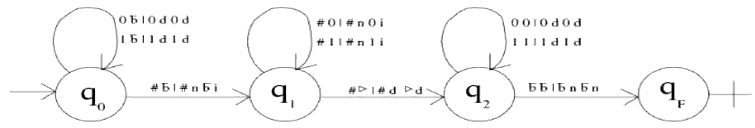
\includegraphics[width=0.8\textwidth]{t8-1.png}

&  Nótese que, ahora, las transiciones están etiquetadas con más información. La parte de la condición tiene ahora el símbolo que hay que leer de la primera cinta y el que hay de leer de la segunda cinta. En la acción indicamos qué símbolo hay que escribir en la primera cinta y adónde mover el cabezal de la primera cinta, y qué símbolo hay que escribir en la segunda cinta y adónde mover el cabezal de la segunda cinta.

& Explicación de la TM:
&& Inicialmente (en $q_0$), copiamos el contenido de la primera cinta en la segunda.

&& Al llegar al separador, pasamos a $q_1$ y regresamos el cabezal de la segunda cinta hasta el principio.

&& A continuación, iniciamos el proceso de comparar ambas palabras en $q_2$. Si la comparación termina satisfactoriamente, vamos a estado aceptador.

& El programa es más sencillo ahora, ya que disponemos de más capacidades. Sin embargo, toda 2-TM se puede simular con una sola TM.

& La idea que usamos es la siguiente: podemos representar el contenido de dos cintas mediante una sola cinta usando un símbolo adicional (\$) para separar ambos contenidos. Uno de los símbolos de la primera cinta quedará marcado de manera especial para recordar que ahí se encuentra el cabezal. Similarmente, uno de los símbolos de la segunda cinta quedará marcado de forma especial para recordar que ahí se encuentra el cabezal (aquí, $a'$ y $b'$).

& Es decir, $\vartriangleright a b \dots b b' a \dots b a \$ b a  \dots b a' a \dots a a \blanco \blanco \blanco \dots$.

& Para simular una transición de la 2-TM, nos veremos obligados a recorrer toda la palabra para ver cuáles son los símbolos apuntados por los cabezales. A continuación, deberemos pasar por ambos cabezales para actualizarlos convenientemente.

& Adicionalmente, puede ocurrir que tengamos que aumentar el tamaño de la palabra izquierda porque estamos accediendo a los blancos del final. Esto nos obligará a \textit{shiftar} la palabra derecha a posiciones más a la derecha.

& Esta idea se puede extender a $k$-TM con más cintas.

\end{easylist}

\subsubsection{Lenguajes de programación}
\begin{easylist}[itemize]

& Pasamos ahora a hablar de lenguajes de programación de más alto nivel.

& Los compiladores convierten lenguajes de programación a lenguajes de bajo nivel de ensamblador dependientes de la arquitectura.

& Estos usan un número limitado de registros ($R_1, \dots, R_n$) y una memoria de forma indexada: $M[0]$, $M[1]$, ...

& Las instruciones son del tipo:

\begin{lstlisting}
    $R_1$ := $R_2$ + $R_3$
    If $R_1$ = 0 Goto Etiqueta
    $R_1$ := $M$[35]
    $M$[13] := $R_5$
    $M$[$R_1$] := $R_2$
    $R_2$ := $M$[$R_1$]
\end{lstlisting}

& Puestos a asumir que trabajamos con memoria infinita, supondremos que, aun cuando contamos con un número finito de registros, la memoria es infinita y que, de hecho, cada registro y cada posición de memoria puede guardar, por ejemplo, un número natural arbitrariamente grande.

& En tal caso, son imprescindibles las instrucciones que involucran acceso indirecto como $M[R_1] \leftarrow R_2$ o $R_2 \leftarrow M[R_1]$, pues si solo pudiésemos acceder solo del modo $M[13] \leftarrow R_5$, solo podríamos acceder a las posiciones de memoria marcadas explícitamente en nuestro programa, y este consta de un número finito de instrucciones.

& Con una máquina de Turing con varias cintas, podemos representar el contenido de cada registro en una cinta distinta. Además, podemos guardar el contenido de toda la memoria en una cinta adicional usando separadores adecuadamente para delimitar el contenido de cada posición que haya sido accedida en algún momento de una ejecución.

& Veremos la instrucción $R_2 \leftarrow M[R_1]$.

& Para simplificar, suponemos que tenemos 3 cintas. La primera representa el contenido $x$ de $R_1$; la segunda, el contenido de $R_2$ que inicialmente está vacía, la tercera representa la memoria con registros guardando palabras sobre 0s y 1s separadas por el símbolo \#.

& Además, asumiremos que, inicialmente, el cabezal de la primera cinta se encuentra al final de $x$, el de la segunda apunta al primer blanco, y el de la tercera apunta al primer separador.

$\vartriangleright\; \dots \; x \; \dots \;  \blanco \;  \blanco\dots$

$\vartriangleright\;  \blanco\;  \blanco\; \dots$

$\vartriangleright\; \#\; w_0 \; \# \; w_1 \; \# \; \dots \; \# \; w_k \;  \blanco \;  \blanco\; \dots$

& La idea será ir avanzando por la memoria al tiempo que restamos 1 unidad al valor de la primera cinta cada vez que pasamos de largo un nuevo separador. En el momento en que la primera cinta ha llegado a 0, sabemos que estamos apuntando a la posición indexada por $x$. Entonces, procederemos a copiar el contenido sobre la segunda cinta.

& El fragmento de grafo de estados es el siguiente.\footnote{Consultad \url{http://youtu.be/fQltYKdFr1E} a partir del minuto 7:25 para ver una descripción del autómata.}

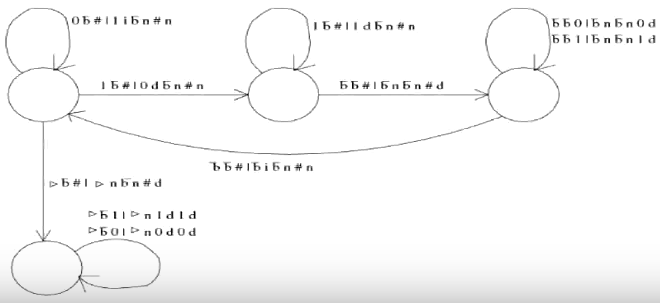
\includegraphics[width=0.8\textwidth]{t8-2.png}

\end{easylist}



\subsection{Asunciones sobre TM y programas}
\subsubsection{Primera asunción}
\begin{easylist}[itemize]
& Consideramos máquina de Turing y programa como sinónimos. Ya hemos justificado anteriormente que las máquinas de Turing pueden simular a cualquier lenguaje de programación; por tanto, nos permitiremos describir procesos en un lenguaje de alto nivel dando por sentado que tenemos su equivalente en TM o que de hecho eso ya es una TM.

& Por ejemplo, este programa es una TM que acepta cualquier entrada:

\begin{lstlisting}
Entrada $x$
       Aceptar
\end{lstlisting}

& Este otro es una TM que, dada una palabra de entrada que codifica un número natural, llega a estado aceptador dejando como resultado en la cinta la codificación del natural resultante de multiplicar por $2$ el que teníamos en la entrada.

\begin{lstlisting}
Entrada $x$
       Salida 2 * $x$
\end{lstlisting}


& Finalmente, este es un programa que decide el lenguaje $\{w \# w\colon w \in\{0,1\}^*\}$.

\begin{lstlisting}
Entrada $w$
    Si $w$ es de la forma $w'\#w'$ entonces Aceptar
    Si no Rechazar
\end{lstlisting}

& Recordemos que este lenguaje concreto ya habíamos visto una TM que lo reconocía.

& Nótese que \verb|Rechazar| corresponde a que la máquina para habiendo llegado a una configuración no aceptadora desde la que no hay transición definida.

\end{easylist}

\subsubsection{Segunda asunción}
\begin{easylist}[itemize]
& Todas las entradas se codifican con números naturales. Los resultados también son números naturales.

& Esto es porque las máquinas codifican toda la información con $0$s y $1$s. Por tanto, es creíble que las entradas y salidas de una máquina se puedan codificar mediante naturales.

& Ejemplos:
&& Entrada $w$ donde $w$ es una palabra. Cuando nos convenga, podremos asumir que recibimos un número natural que codifica una palabra.

&& Entrada $\langle x, y\rangle$. Es decir, una pareja de naturales. También podremos asumir que recibe un natural que codifica una palabra de naturales.

&& También se pueden representar una CFG $G$, un DFA $A$ o una terna con dos palabras y un sistema de reescritura: $\langle u, v, R = \{u_1 \to v_1, \dots, u_n \to v_n\}\rangle$.

\end{easylist}

\subsubsection{Tercera asunción}
\begin{easylist}[itemize]
& Cuando nos convenga, asumiremos que nuestro sistema de codificación enumera todas las entradas correctas.

& Por ejemplo, el conjunto de todos los DFA que son mínimos. Lo podemos ver como un conjunto de naturales que codifican DFA. En general, el complementario de este conjunto contendría: por un lado, a los naturales que codifican DFA no mínimos y a los naturales que no codifican correctamente ningún DFA.

& Si asumimos que el sistema de codificación asocia a cada natural un DFA de manera biunívoca, entonces el complementario es el que aparece a la derecha de la igualdad. $\{A \in \textrm{DFA} \colon A \textrm{ es mínimo}\} = \overline{\{A \in \textrm{DFA}\colon A \textrm{ no es mínimo}\}}$.

& Lo mismo sucede para ternas $\langle u, v, R\rangle$.

\end{easylist}


\subsubsection{Cuarta asunción}
\begin{easylist}[itemize]
& El conjunto de todos los programas se puede enumerar mediante los números naturales, ya que nuestros programas quedan almacenados mediante $0$s y $1$s. Asumimos una codificación fija concreta, sin especificar cuál; pues es irrelevante cuál sea mediante enumere a todos los programas posibles y sea codificable y descodificable algorítmicamente.

& Bajo esta suposición, mediante $M_n$ denotaremos a la máquina codificada por el número natural $n$.

& Esto puede ocasionar ambigüedad, pues $M_1$ significará la máquina $1$ o bien la máquina codificada por 1. El contexto soluciona esta ambigüedad.

\end{easylist}


\subsubsection{Quinta asunción}
\begin{easylist}[itemize]
& Podemos ejecutar programas desde otros programas. Es decir, existe un intérprete $U$ capaz de simular la ejecución de otro programa con una cierta entrada. Esta asunción es natural, pues se trata de la idea básica de los intérpretes y compiladores.

& Por ejemplo, este programa recibe un natural que codifica a dos naturales $\langle x, y\rangle$, simula la ejecución del programa codificado por $x$ con entrada $y$ y da como salida la misma salida de dicha ejecución. Esta no es más que una posible implementación de la máquina universal usando una instrucción que, de hecho, asume ya otra implementación de la máquina universal. Por supuesto, esta máquina se queda colgada con una entrada si esta ejecución no para.

$U(\langle x, y\rangle) = M_x(y)$

\begin{lstlisting}
Entrada $\langle x, y \rangle$
       Salida $M_x(y)$
\end{lstlisting}

& En este otro ejemplo ejecutamos el intérprete solo durante 100 pasos. Así, podemos ejecutar un intérprete por tiempo limitado. Podemos asumir que, con un paso, nos referimos a una transición de la TM.

\begin{lstlisting}
Entrada $\langle x, y \rangle$
       Si $M_x(y)$ para en 100 pasos, entonces Salida $M_x (y)$
       Si no, entonces Salida 0
\end{lstlisting}

& Para cada número natural $n$, con $\varphi_n$ denotamos la función computada por la máquina codificada por $n$: $\varphi_n \equiv \varphi_{M_n}$; y con $\mathcal L_n$, denotamos el lenguaje aceptado por la máquina codificada por $n$: $\mathcal L_n = \mathcal L(M_n)$.

& Nótese que, cuando la función computada por $n$ está definida para un cierto $m$ (esto es, $\varphi_n(m) \downarrow$), la máquina codificada por $n$ con entrada $m$ da el mismo resultado: $\varphi_n(m) = M_n(m)$.

& Pero, recuérdese que, aun cuando la función no esté definida, la máquina puede parar llegando a una configuración terminal no aceptadora ($\varphi_n(m) \uparrow$ o $M_n(m)  \downarrow$).

& De hecho, $M_n$ y $\varphi_n$ son objetos muy distintos.

& Por ejemplo, sea $n$ el número que codifica el programa

\begin{lstlisting}
Entrada $x$
    Salida 2 * $x$
\end{lstlisting}

& Tenemos que $M_n$ es justamente el programa (el bloque de código); en cambio, $\varphi_n$ es la función que implementa. Es decir: $M_n \neq \varphi_n = \{(0,0), (1,2), (2,4), \dots\}$.

& En el caso en que $n$ codifique a un programa que para siempre y rechaza o a un programa que no para con ninguna entrada, $\varphi_n$ es el conjunto vacío ($M_n \neq \varphi_n = \varnothing$) también llamada \textit{función vacía} o \textit{totalmente indefinida}.

\begin{lstlisting}
Entrada $x$
       Rechazar
\end{lstlisting}

\begin{lstlisting}
Entrada $x$
       Colgarse
\end{lstlisting}

& Podemos ahora redefinir nociones que ya habíamos introducido.

& Un subconjunto $C \subseteq N$ de los naturales es decible si existe un natural tal que la máquina que codifica lo reconoce y para con toda entrada: $C \in \textrm{Dec} \equiv \exists x \colon (\textrm{Dom}(\varphi_x) = C \land \forall y \colon M_x(y) \downarrow)$.

& Un subconjunto $C \subseteq N$ de los naturales es semi-decible si existe un natural tal que la máquina que lo codifica lo reconoce: $C \in \textrm{semi-Dec} \equiv \exists x \colon \mathcal L_x = C$.

& Una función es computable si existe un natural tal que, la máquina que lo codifica, la computa: si $f \colon \mathbb N \to \mathbb N$, entonces $f$ es computable si $\exists x \colon \varphi_x = f$.

\end{easylist}

\subsection{Operaciones sobre TM y programas}
\textit{Falta redactarlo}
\begin{easylist}[itemize]
\end{easylist}
\end{document}
